\documentclass[12pt,a4paper,titlepage]{article}

\usepackage{vmargin}
\setpapersize{A4}
%            left      right       headheight  footheight
%                 top       bottom      headskip  footskip
\setmarginsrb{2cm}{2cm}{2cm}{2cm}{0pt}{0mm}{0pt}{15mm}

%\usepackage[nomarkers]{endfloat}
\usepackage{natbib}
\usepackage[dvips]{graphicx}
\usepackage{color}
\usepackage{tabularx}
\usepackage{multicol}
\usepackage{mathptmx,helvet,courier}


\usepackage[ps2pdf,breaklinks=true,colorlinks=false,a4paper=true]{hyperref}
\hypersetup{
pdfauthor = {Patrick Samuelsson, Stefan Gollvik, Christer Jansson, Ekaterina Kourzeneva, Willem Jan van de Berg},
pdftitle = {The land-surface scheme and lake model of the Rossby Centre regional atmospheric climate model (RCA4)},
pdfsubject = {SMHI Meteorologi},
pdfcreator = {LaTeX with hyperref package},
pdfproducer = {dvips + ps2pdf}}

\newcommand{\empr}{\\ [0.5 cm]}
\newcommand{\nlem}{\mbox{}\\[0.5 cm]}
\newcommand{\Frac}{\displaystyle \frac}
\def\del[#1]#2{\displaystyle \frac {\partial #1}{\partial #2}}
\def\delt[#1]#2{\displaystyle {\partial #1}/{\partial #2}}
\def\deg{$^\circ$}
\def\appr{$\sim$}
\def\ms{m s$^{-1}$}

\setlength{\parindent}{0cm}
\setlength{\parskip}{2mm}


\begin{document}

\bibliographystyle{elsart-harv-mod}

%%%%%%%%%%%%%%%%%%%%%%%%%%%%%%%%%%%%%%
\begin{figure}[!b]
\centerline{
 \includegraphics[width=12cm, trim=140 330 140 -170]{figures/rca3_lss_frontpage.prn}}
\end{figure}
%%%%%%%%%%%%%%%%%%%%%%%%%%%%%%%%%%%%%%


%\title{Parameterization of land-surface processes
%on hourly to inter-annual timescales in a regional climate model}
\title{The land-surface scheme and lake model of the Rossby Centre regional atmospheric climate model (RCA4)}
\author{Patrick Samuelsson, Stefan Gollvik, Christer Jansson, Marco Kupiainen, \\
Ekaterina Kourzeneva, Willem Jan van de Berg \\
\ \\
Rossby Centre, Swedish Meteorological and Hydrological Institute \\
SE-601 76 Norrk\"oping, Sweden\\
\ \\
Meteorologi, 1xx}
%\date{2011}


\maketitle

\begin{abstract}
This report describes the physical processes as part of the Land-Surface Scheme (LSS) in the Rossby Centre Regional Atmospheric
Climate Model (RCA4). The LSS is a tiled scheme with the three main tiles with respect to temperature:
forest, open land, and snow. The open land tile is divided into a vegetated and a bare soil part for latent heat flux calculations. The individual fluxes of heat and momentum from these tiles are weighted in order to obtain grid-averaged values at the lowest atmospheric model level according to the fractional areas of the tiles. The forest tile is internally divided into three sub-tiles: forest canopy, forest floor soil, and snow on forest floor. All together this gives three to five different surface energy balances depending on if snow is present or not.

The soil is divided into five layers with respect to temperature, with a no-flux boundary condition at three meters depth, and into three layers
with respect to soil moisture, with a maximum depth defined by the root depth as given by physiography database.
Runoff generated at the bottom of the deep soil layer may be used as input to a routing scheme.

In addition to the soil moisture storages there are six more water storages in the LSS: interception of water on open land vegetation and on forest canopy, snow water equivalent of open land and forest snow, and liquid water content in both snow storages.

Diagnostic variables of temperature and humidity at 2m and wind at 10m are calculated individually for each tile.
\end{abstract}

\newpage

\tableofcontents

\newpage

%%%%%%%%%%%%%%%%%%%%%%%%%%%%%%%%%%%%%%%%%%%%%%%%%%%%%%%%%%%%%%%%%%%%%%%%%%%%%%%%%%%%%%%%%%%%%
%%%%%%%%%%%%%%%%%%%%%%%%%%%%%%%%%%%%%%%%%%%%%%%%%%%%%%%%%%%%%%%%%%%%%%%%%%%%%%%%%%%%%%%%%%%%%

\section{Introduction}

This report documents the Land-Surface Scheme (LSS) of the fourth version of the Rossby Centre Regional Atmospheric
Climate Model (RCA4). For a general description of the role of a LSS in a regional climate model and for
documentataion of the LSS in RCA3 please refer to  \cite[]{kn:Samuelsson06}.
Here all the specific details of \cite[]{kn:Samuelsson06} are kept but modified with any updates made. In additon
the changes introduced in the LSS between RCA3 and RCA4 are documenetd. The changes concern in general:
\begin{itemize}
\item New physiography based on ECOCLIMAP (\ref{}).
\item Number of soil layers with respect to soil moisture are increased from two to three where the thickness of the third 
layer is defined by the root depth from ECOCLIMAP. There is also separate soil columns with respect to
soil water under forest and open land, respectively (\ref{}).
\item Exponetial root distribution is used with compensation for very dry soil conditions (Section \ref{sec:rootdistribution}).
\item Density of organic carbon is used to modify heat conduction and heat capacity of the soil (\ref{}).
\item FLake is introduced as lake model and lake depth is defined from a global lake-depth data base (\ref{}).
\item Prognostic snow albedo is modified to perform better in cold-climate conditions (\ref{}).
\end{itemize}

%%%%%%%%%%%%%%%%%%%%%%%%%%%%%%%%%%%%%%
\begin{figure}[!tbp]
\centerline{
 \includegraphics[angle=-90, width=12.5cm, trim=100 100 100 100]{figures/rca4_lss.prn}}
 \caption{A principal sketch of the land-surface scheme in RCA4. The LSS is divided into three main tiles: forest ($A_{for}$),
 open land ($A_{opl}$) and snow on open land ($A_{sn}$). The forest also has a snow sub-tile ($A_{forsn}$). Prognostic
 temperatures are marked in red while the water prognostic variables are marked in blue. Each individual tile is connected to the lowest atmospheric
 level via their corresponding aerodynamic resistances ($r_{a}$). For evapotranspiration calculations a number of surfaces resistances
 are used ($r_{s}$).} 
\setlength{\columnsep}{0pt}
\begin{multicols}{2}
\begin{scriptsize}
\begin{tabularx}{\linewidth}{|lm{4.5cm}l}
{\bf Parameter}	& {\bf Definition}				& {\bf Reference} \\
\hline
\multicolumn{3}{|l}{\bf Sub-grid fractions} \\
\hline
$A_{for}$	& fractional area of forest  \\
$A_{opl}$	& fractional area of open land \\
$A_{sn}$	& fractional area of open-land snow		& Sec \ref{sec:snowcover} \\
$A_{forsn}$	& fractional area of snow in forest		& Sec \ref{sec:snowcover} \\
\hline
\multicolumn{3}{|l}{\bf Prognostic temperatures} \\
\hline
$T_{opls}$	& open land soil surface temperature \\
$T_{sn}$	& snow surface temperature			& Eq \ref{tsnow} \\
$T_{sns}$	& soil temperature below snow \\
$T_{forsn}$	& forest snow surface temperature		& Eq \ref{eq:fortemp} \\
$T_{fors}$	& forest soil surface temperature		& Eq \ref{eq:fortemp} \\
$T_{forsns}$	& soil temperature below forest snow \\
$T_{forc}$	& forest canopy temperature			& Eq \ref{eq:fortemp} \\
\hline
\multicolumn{3}{|l}{\bf Prognostic water storages} \\
\hline
$sn$		& open land snow water equivalent		& Sec \ref{sec:snow} \\
$sn_{for}$	& forest snow water equivalent			& Sec \ref{sec:snow} \\
$w_{oplv}$	& intercepted water on low vegetation		& Sec \ref{sec:interc} \\
$w_{forc}$	& intercepted water on forest canopy		& Sec \ref{sec:interc} \\
$w_{sn}$	& snow liquid water				& Sec \ref{sec:snow} \\
$w_{forsn}$	& forest snow liquid water			& Sec \ref{sec:snow} \\
\hline
\end{tabularx}

\begin{tabularx}{\linewidth}{|lm{4.5cm}l|}
\cline{1-3}
{\bf Parameter}	& {\bf Definition}				& {\bf Reference} \\
\cline{1-3}
\multicolumn{3}{|l|}{\bf Resistances} \\ 
\cline{1-3}
$r_{svfor}$	& forest canopy surface resistance		&  Eq \ref{eq:rsv} \\ 
$r_{svopl}$	& open land vegetation surface resistance	&  Eq \ref{eq:rsv} \\
$r_{ssfor}$	& forest floor soil surface resistance 		& Eq \ref{eq:rss} \\
$r_{ssopl}$	& open land soil surface resistance 		& Eq \ref{eq:rss} \\
$r_{afor}$	& aerodynamic resistance above forest 		& Sec \ref{sec:ra} \\
$r_{aopl}$	& aerodynamic resistance above open land 	& Sec \ref{sec:ra} \\
$r_{asn}$	& aerodynamic resistance above snow 		& Sec \ref{sec:ra} \\ 
$r_{b}$		& aerodynamic resistance (forest canopy - canopy air) & Eq \ref{eq:condrb} \\
$r_{d}$		& aerodynamic resistance (forest floor - canopy air)  & Eq \ref{eq:rd} \\
\cline{1-3}
\multicolumn{3}{|l|}{\bf Depth of soil layers} \\ 
\cline{1-3}
$z_{T1}$--$z_{T5}$ & thickness of soil layers w.r.t. temperature (0.01, 0.062, 0.21, 0.72, 1.89 m)	&   \\ 
$z_{\theta 1}$--$z_{\theta 3}$ & thickness of soil layers w.r.t. soil moisture (0.072, 0.21 m, root depth - 0.282) &   \\ 
\cline{1-3}

\end{tabularx}
\end{scriptsize}
\end{multicols}
\label{lssfig}
\end{figure}
%%%%%%%%%%%%%%%%%%%%%%%%%%%%%%%%%%%%%%


%%%%%%%%%%%%%%%%%%%%%%%%%%%%%%%%%%%%%%%%%%%%%%%%%%%%%%%%%%%%%%%%%%%%%%%%%%%%%%%%%%%%%%%%%%%%%
%%%%%%%%%%%%%%%%%%%%%%%%%%%%%%%%%%%%%%%%%%%%%%%%%%%%%%%%%%%%%%%%%%%%%%%%%%%%%%%%%%%%%%%%%%%%%

\section{Specific LSS processes}


\subsection{Heat fluxes and aerodynamic resistance}
\label{sec:ra}

The sensible ($H$) and
latent ($E$) heat fluxes between the surface and the first atmospheric level at height $z_{am}$
($\sim$90 m in a set-up with 24 vertical levels) are parameterized as

%%%%%%%%%%%%%%%%%%%%%%%%
\begin{equation}
H = \rho c_p \frac{T_s - T_{am}}{r_a}
\label{eq:H}
\end{equation} 
%%%%%%%%%%%%%%%%%%%%%%%%%

 and

%%%%%%%%%%%%%%%%%%%%%%%%
\begin{equation}
E = \rho L_e \frac{q_s(T_s) - q_{am}}{r_a + r_s}.
\label{eq:E}
\end{equation} 
%%%%%%%%%%%%%%%%%%%%%%%%%

Here, $\rho$ is air density, $c_p$ is heat capacity of the air,
$L_e$ is latent heat of vaporisation of water, $T_s$ is surface temperature, $T_{am}$ is temperature at $z_{am}$,
$q_s$ is surface saturated specific humidity, $q_{am}$ is specific humidity at $z_{am}$ and
$r_a$ aerodynamic resistance. The formulation of the surface resistance $r_s$
depends on the surface as described in Section \ref{sec:surfres}.
%for snow and intercepted water it is zero, for bare soil it is formulated according
%to \cite{kn:vdHurk00}, and for vegetation according to \cite{kn:Noilhan89}.

The aerodynamic resistance is important for both fast response processes such as diurnal temperature
range and for long term performance such as a correct division of precipitation into evapotranspiration and runoff.
The LSS has three different aerodynamic resistances represented by the characteristics of forest, open land,
and snow, with respect to surface temperature and roughness lengths of momentum and heat.
The aerodynamic resistance for heat is given by the drag coefficient, $C_h$:

%%%%%%%%%%%%%%%%%%%%%%%%
\begin{equation}
C_h = \frac{1}{u r_a} = \frac{k^2}{\ln(z_{am}/z_{0m})\ln(z_{am}/z_{0h})}   f_h(Ri,z_{am}/z_{0h}),
\label{eq:Ch}
\end{equation} 
%%%%%%%%%%%%%%%%%%%%%%%%%

where $u$ is wind speed at $z_{am}$, $k$ is the von Karman's constant, $z_{0m}$ and $z_{0h}$ are roughness lengths
for momentum and heat, respectively, $Ri$ is the Bulk-Richardson number and $f_h$ represents analytic stability functions based on modified \cite{kn:Louis82} formulations.

The dependence of the heat fluxes on the aerodynamic resistance is strong. This 
in turn has been shown to be quite sensitive to the ratio between the roughness length of heat and momentum
\cite[]{kn:Beljaars94,kn:Chen97,kn:Samuelsson03,kn:vdHurk02}.
However, the problem is that estimations of the ratio $z_{0m}/z_{0h}$ vary considerably. According to \cite{kn:Chen97}
it is reasonable to relate the ratio to the properties of the flow as suggested by \cite{kn:Zilitinkevich95}:


%%%%%%%%%%%%%%%%%%%%%%%%
\begin{equation}
\frac{z_{0m}}{z_{0h}} = \exp(k C \sqrt{Re^*}),
\label{eq:zmzh}
\end{equation} 
%%%%%%%%%%%%%%%%%%%%%%%%%

where

%%%%%%%%%%%%%%%%%%%%%%%%
\begin{equation}
Re^* = \frac{u_0^* z_{0m}}{\nu},
\label{eq:Rest}
\end{equation} 
%%%%%%%%%%%%%%%%%%%%%%%%%

where $\nu$ is the kinematic molecular viscosity, $Re^*$ is the roughness Reynolds number, and $u_0^*$ is the
surface friction velocity. $C$ is an empirical constant which \cite{kn:Chen97} estimated to be 0.1
based on comparisons between simulations and observations of heat fluxes.
$r_a$ is sensitive to the value of $C$ for large values on $z_{0m}$ ($>0.2$ m) and
to the value of $z_{0m}$ for small values on $z_{0m}$ ($<0.1$ m).
However, the Zilitinkevich formulation gives too low heat fluxes over land in RCA.
For the surface fluxes to be reasonably we set $z_{0h}=z_{0m}=\max( 0.2, z_{0m,ECO} )$ m for snow free open land,
where $z_{0m,ECO}$ represent momentum roughness as given from ECOCLIMAP (\ref{}).
The Zilitinkevich formulation of the ratio $z_{0m}/z_{0h}$ is used only for snow surfaces with $z_{0m}=0.002$ m.
For forest we use $z_{0h}=z_{0m}$ as suggested by \cite{kn:Molder99b}, which also gives good
results when comparing simulated and observed heat fluxes.

%%%%%%%%%%%%%%%%%%%%%%%%%%%%%%%%%%%%%%%%%%%%%%%%%%%%%%%%%%%%%%%%%%%%%%%%%%%%%%%%%%%%%%%%%%%%%
%%%%%%%%%%%%%%%%%%%%%%%%%%%%%%%%%%%%%%%%%%%%%%%%%%%%%%%%%%%%%%%%%%%%%%%%%%%%%%%%%%%%%%%%%%%%%

\subsection{Interception of rain on vegetation}
\label{sec:interc}

Rain intercepted by the vegetation is available for potential evaporation which means that it has a strong influence on the fluxes of heat and consequently also on the surface temperature. Interception of snow is not included.
Below freezing ($T_{forc}\leq0$\deg C) rain is intercepted. Any water present will stay on the vegetation and evaporate as super-cooled water. The parameterization of interception of rain follows \cite{kn:Noilhan89} and its implementation into RCA4
is similar to the implementation in RCA2 as described by \cite{kn:Bringfelt01}. The rate of change of intercepted
water is described by

%%%%%%%%%%%%%%%%%%%%%%%%%
\begin{equation}
\label{interc}
\frac{w_{veg}^{\tau+1}-w_{veg}^{\tau}}{\Delta t} = \mathrm{veg} (P - \frac{\delta}{L_e}E_v),
\end{equation}
%%%%%%%%%%%%%%%%%%%%%%%%%

where $w_{veg}$ is amount of intercepted water (mm of water on the specified fraction), $\tau$ and
$\tau+1$ represent present and next time step, $\Delta t$ is the length of the time step (s),
$\mathrm{veg}$ is a vegetation cover parameter, $P$ is rain intensity (kg m$^{-2}$ s$^{-1}$), $E_v$ is evaporation
of intercepted water (W m$^{-2}$), and $\delta$ is the fraction of of the
vegetation covered with water defined as \cite[]{kn:Deardorff78}

%%%%%%%%%%%%%%%%%%%%%%%%%
\begin{equation}
\label{delta}
\delta = \left( \frac{w_{veg}}{w_{vegmax}} \right)^{2/3}.
\end{equation}
%%%%%%%%%%%%%%%%%%%%%%%%%

The exponent $2/3$ comes from the fact that the intercepted water exists in the form
of droplets where the water volume of the droplets
is proportional to $r^3$, where $r$ is the radius of the droplets, and the surface of the droplets is proportional to $r^2$.
$w_{vegmax}=0.2\cdot \mathrm{veg} \cdot \mathrm{LAI}$ is the maximum amount of water allowed on the vegetation
\cite[]{kn:Dickinson84}. Here LAI is the leaf area index as defined in Section \ref{sec:surfres}.

The evaporation $E_v$ is calculated according to

%%%%%%%%%%%%%%%%%%%%%%%%
\begin{equation}
E_v = \rho L_e \frac{q_s(T_s) - q_{am}}{r_a}.
\label{eq:Ev}
\end{equation} 
%%%%%%%%%%%%%%%%%%%%%%%%%

To keep the solution numerically stable $\delta$ is solved implicitly

%%%%%%%%%%%%%%%%%%%%%%%%%
\begin{equation}
\label{deltamean}
\delta = (1-\alpha) \left(\frac{w_{veg}^{\tau}}{w_{vegmax}}\right)^{2/3} + \alpha \left(\frac{w_{veg}^{\tau+1}}{w_{vegmax}}\right)^{2/3},
\end{equation}
%%%%%%%%%%%%%%%%%%%%%%%%%

where $\alpha$ represents the degree of implicitly (set to 0.5).
$w_{veg}^{\tau+1}$ is found by replacing $\delta$ in Equation \ref{interc} with Equation \ref{deltamean}.
The resulting equation is solved using the Newton-Raphson's method.

The new value of intercepted water amount may not exceed the maximum value. Thus, any excess water becomes
throughfall, $thr = \max(0.0, (w_{veg}^{\tau+1} - w_{vegmax})/\Delta t)$. The final water amount is corrected
with the throughfall as $w_{veg}^{\tau+1} = w_{veg}^{\tau+1} - thr \cdot \Delta t$ and
the total amount of rain that falls to the ground becomes
$P_{tot} = thr + (1.0 - \mathrm{veg}) P$.

This parameterization is used for interception of rain on both forest canopy and on open land vegetation
with individual values for the parameters $\mathrm{veg}$ and $\mathrm{LAI}$.
In the forest case $T_s=T_{forc}$, $q_{am}=q_{fora}$, and $r_a=r_b$ and in the open land case 
$T_s=T_{opls}$ and $r_a=r_{aopl}$.

%%%%%%%%%%%%%%%%%%%%%%%%%%%%%%%%%%%%%%%%%%%%%%%%%%%%%%%%%%%%%%%%%%%%%%%%%%%%%%%%%%%%%%%%%%%%%
%%%%%%%%%%%%%%%%%%%%%%%%%%%%%%%%%%%%%%%%%%%%%%%%%%%%%%%%%%%%%%%%%%%%%%%%%%%%%%%%%%%%%%%%%%%%%

\subsection{Surface resistances}
\label{sec:surfres}

For latent heat flux a surface resistance is added for vegetation transpiration
and for bare soil evaporation. Snow surfaces and intercepted water have zero
surface resistance. In the case of
condensation, $q_s(T_s)<q_{am}$, the surface resistance is also put to zero.

The vegetation surface resistance, closely following
\cite{kn:Noilhan89}, is a function of a vegetation dependent minimum surface
resistance, $r_{svmin}$, the LAI, and five factors representing ($F_1$) the influence of
photosynthetically active radiation, ($F_2$) the effect of water stress, ($F_3$) the effect of
vapor pressure deficit, ($F_4$) an air temperature dependence, and ($F_5$) a soil temperature dependence:

%%%%%%%%%%%%%%%%%%%%%%%%%
\begin{equation}
  \label{eq:rsv}
  r_{sv} = \frac{r_{svmin}}{\mathrm{LAI}} F_1 F_2^{-1} F_3^{-1} F_4^{-1} F_5^{-1}.
\end{equation}
%%%%%%%%%%%%%%%%%%%%%%%%%

The photosynthetically active radiation is assumed to be $0.55 S\!\!\downarrow$, where $S\!\!\downarrow$ is
the incoming shortwave radiation. The factor $F_1$ is defined as

%%%%%%%%%%%%%%%%%%%%%%%%%
\begin{equation}
  \label{eq:F1}
  F_1 = \frac{1+f}{f+r_{svmin}/r_{svmax}},
\end{equation}
%%%%%%%%%%%%%%%%%%%%%%%%%

with

%%%%%%%%%%%%%%%%%%%%%%%%%
\begin{equation}
  \label{eq:f}
  f = 0.55 \frac{S\!\!\downarrow}{S_L}\frac{2}{\mathrm{LAI}},
\end{equation}
%%%%%%%%%%%%%%%%%%%%%%%%%

where $r_{svmax}$ is a maximum surface resistance set to 5000 s m$^{-1}$ and $S_L$ is a limit value of 30 W m$^{-2}$
for a forest and of 100 W m$^{-2}$ for a crop.

The factor $F_2$ varies between 0 and 1 depending on available soil moisture $\theta$:

%%%%%%%%%%%%%%%%
\begin{equation}
\label{eq:F2}
F_2 = \left\{
\begin{array}{l l}
1,							& \mbox{if $\theta > \theta_{cr}$} \\
\Frac{\theta - \theta_{wi}}{\theta_{cr}-\theta_{wi}},	& \mbox{if $\theta_{wi} \leq \theta \leq \theta_{cr}$} \\
0,							& \mbox{if $\theta < \theta_{wi}$} \\
\end{array}
\right.
\end{equation}
%%%%%%%%%%%%%%%%

where $\theta_{wi}$ is the wilting point, $\theta_{cr}=0.9 \theta_{fc}$ and $\theta_{fc}$ is the field capacity. To account for different
soil moisture conditions in different root layers the factor $F_2$ is calculated
individually for each soil layer which in combination with the other factors actually gives
different $r_{sv}$-values for each soil layer. These $r_{sv}$-values are finally weighted with respect
to the depth of each soil layer (see Appendix \ref{sec:weightsurfres}).

Factor $F_3$ represents the effect of vapor pressure deficit of the atmosphere or, as
expressed here, in terms of specific humidity
\cite[]{kn:Jarvis76,kn:Sellers86}:

%%%%%%%%%%%%%%%%%%%%%%%%%
\begin{equation}
  \label{eq:F3}
  F_3 = 1-g(q_s(T_s)-q_{am}),
\end{equation}
%%%%%%%%%%%%%%%%%%%%%%%%%

where $g$ is a vegetation-dependent empirical parameter set to 0.04 for a forest and to zero for a crop.
In the forest case $T_s=T_{forc}$ and $q_{am}=q_{fora}$ and in the open land case 
$T_s=T_{opls}$.

The air temperature has a strong influence on the transpiration with the most
favorable conditions at 25\deg C. The factor $F_4$ describes the air temperature
dependence following \cite{kn:Dickinson84}

%%%%%%%%%%%%%%%%%%%%%%%%%
\begin{equation}
  \label{eq:F4}
  F_4 = 1.0-0.0016(298.0-T_{am})^2,
\end{equation}
%%%%%%%%%%%%%%%%%%%%%%%%%

where $T_{am}=T_{fora}$ in the forest case.

The vegetation does not become active in spring until
the soil temperature in the root zone reaches at least +2\deg C.
Therefore, an additional factor, $F_5=1-f(T)$, is added which varies between 0 and 1 for soil temperatures between
$T_1=T_{melt}+4$ K and $T_2=T_{melt}+2$ K following a sinusoidal function originally intended for parameterization
of soil freezing as described in \cite{kn:Viterbo99}:

%%%%%%%%%%%%%%%%
\begin{equation}
\label{eq:fTV}
f(T) = \left\{
\begin{array}{l l}
0,										& \mbox{$T>T_1$} \\
0.5\left[ 1-\sin\left( \Frac{\pi(T-0.5T_1-0.5T_2)}{T_1-T_2} \right) \right],	& \mbox{$T_2 \le T \le T_1$} \\
1,										& \mbox{$T < T_2$.} \\
\end{array}
\right.
\end{equation}
%%%%%%%%%%%%%%%%

As for $F_2$, this gives different $F_5$-values for different soil layers depending on their
temperature.

For RCA, ECOCLIMAP provides separate leaf area indexes (LAI) for open land vegetation, for coniferous forest and for broadleaved forest.
An options exists to diagnostically calculate LAI during the simulation
The coniferous forest LAI, $\mathrm{LAI}_{cf}$, is set constant to $4.0$ while the open land vegetation
and deciduous forest LAIs are parameterised as functions of soil temperature \cite[]{kn:Hagemann992}:

%%%%%%%%%%%%%%%%%%%%%%%%%
\begin{equation}
\mathrm{LAI}_T = \mathrm{LAI}_{min} + f(T_{soil}) (\mathrm{LAI}_{max} - \mathrm{LAI}_{min}),
\label{eq:LAI1}
\end{equation}
%%%%%%%%%%%%%%%%%%%%%%%%%

where

%%%%%%%%%%%%%%%%%%%%%%%%%
\begin{equation}
f(T_{soil}) = 1 - \left( \frac{T_{max}-T_{soil}}{T_{max}-T_{min}} \right)^2.
\label{eq:Tsoil}
\end{equation}
%%%%%%%%%%%%%%%%%%%%%%%%%

The allowed range in LAI, defined by the maximum and minimum values LAI$_{max}$ and LAI$_{min}$, are set to 0.4--2.3
for open land vegetation and to 0.4--4.0 for deciduous forest, respectively. LAI does not show sub-diurnal variability.
Thus, the soil temperature, $T_{soil}$, in Equation
\ref{eq:Tsoil} has to be unaffected by diurnal variations why we have chosen the temperature in the fourth soil layer.
The minimum and maximum temperatures, $T_{min}$ and $T_{max}$, are set to 273.0 and 293.0 K, respectively.
All LAI values are set to LAI$_{min}$ for soil moisture values $\theta_s\leq\theta_{wi}$, where $\theta_{wi}$ is the wilting point.

%In dry climate regions the LAI may also be affected by the soil water availability. To take this effect into
%account the leaf area index due to soil temperature in Equation \ref{eq:LAI1} is modified to give the final LAI
%according to
%
%%%%%%%%%%%%%%%%%%%%%%%%%%
%\begin{equation}
%\mathrm{LAI} = \mathrm{LAI}_T \left[ 1 - \exp\left( -5 \frac{\theta - \theta_{wi}}{\theta_{fc} - \theta_{wi}} \right) \right].
%\label{eq:LAI2}
%\end{equation}
%%%%%%%%%%%%%%%%%%%%%%%%%%
%
%This relationship has not yet been thoroughly validated against observed LAI values but only adjusted
%to give a reasonable reduction in LAI due to drying soil.

Bare soil evaporation is restricted by the soil surface resistance \cite[]{kn:vdHurk00}:

%%%%%%%%%%%%%%%%%%%%%%%%%
\begin{equation}
  \label{eq:rss}
  r_{ss} = \frac{r_{ssmin}}{1-f(T)}\frac{\theta-\theta_{wi}}{\theta_{fc} - \theta_{wi}},
\end{equation}
%%%%%%%%%%%%%%%%%%%%%%%%%

where $r_{ssmin}$ represents a minimum value of the surface resistance ($=50$ sm$^{-1}$).
As described in Section \ref{sec:soiltemp} there is no solid phase of soil water, therefore,
$1-f(T)$ is used to represent the fraction of liquid soil water to total soil water in the top soil
layer with $T_1=T_{melt}+1$ K and $T_2=T_{melt}-3$ K.


%%%%%%%%%%%%%%%%%%%%%%%%%%%%%%%%%%%%%%%%%%%%%%%%%%%%%%%%%%%%%%%%%%%%%%%%%%%%%%%%%%%%%%%%%%%%%
%%%%%%%%%%%%%%%%%%%%%%%%%%%%%%%%%%%%%%%%%%%%%%%%%%%%%%%%%%%%%%%%%%%%%%%%%%%%%%%%%%%%%%%%%%%%%

\subsection{Evapotranspiration}

In the case of wet vegetation the total evapotranspiration is the sum of evaporation of intercepted water,
$E_v$ in Equation \ref{eq:Ev}, and transpiration via stomata, as expressed through Equation \ref{eq:E}. 
The total evapotranspiration, $E_c$, is defined as

%%%%%%%%%%%%%%%%%%%%%%%%%
\begin{equation}
  \label{eq:Ec}
E_c = \rho L_e h_v \frac{q_s(T_s) - q_{am}}{r_a + r_{sv}},
\end{equation}
%%%%%%%%%%%%%%%%%%%%%%%%%

where the Halstead coefficient, $h_v$, includes the fraction of the vegetation covered with water, $\delta$,

%%%%%%%%%%%%%%%%%%%%%%%%%
\begin{equation}
\label{eq:hv}
h_v = h_v^{tr} + h_v^{int} = (1-k\delta) + \frac{r_a + r_{sv}}{r_a} k\delta.
\end{equation}
%%%%%%%%%%%%%%%%%%%%%%%%%

The coefficient is subdivided into a transpiration part, $h_v^{tr}$, and into an interception part, $h_v^{int}$.
The Halstead coefficient, as defined in \cite{kn:Noilhan89}, is modified by introducing the
factor $k$ to take into account the fact that also saturated vegetation can transpire, i.e. when
$\delta=1$ \cite[]{kn:Bringfelt01}. k=0 would represent a situation where the intercepted water forms full spheres just
touching the vegetation surface and therefore allow full transpiration from the whole leaf
surface. k=1 would represent a situation where a water film covers the vegetation completely
and no transpiration is allowed. To adhere the interception model as described above, where the
intercepted water exists as droplets, we set the value of $k$ to $0.25$. Note that in the case
of condensation, i.e. $E_c<0$, $h_v=(r_a + r_{sv})/r_a$.


%%%%%%%%%%%%%%%%%%%%%%%%%%%%%%%%%%%%%%%%%%%%%%%%%%%%%%%%%%%%%%%%%%%%%%%%%%%%%%%%%%%%%%%%%%%%%
%%%%%%%%%%%%%%%%%%%%%%%%%%%%%%%%%%%%%%%%%%%%%%%%%%%%%%%%%%%%%%%%%%%%%%%%%%%%%%%%%%%%%%%%%%%%%

\subsection{Forest processes}

The forest canopy is characterized by low heat capacity which means that its temperature responds
fast to changes in fluxes. Thus, to realistically simulate diurnal variations in 2m-temperature in a
forest dominated landscape this effect must be accounted for. The forest canopy acts more or less
like a cover above the forest floor, therefore, it is really the temperature and specific humidity conditions
in the canopy air space, $T_{fora}$ and $q_{fora}$, that set the conditions for heat fluxes between forest canopy, forest floor,
and lowest model level in the forest tile. $T_{fora}$ and $q_{fora}$ are diagnostic variables which have
to be solved iteratively as described in Appendix \ref{sec:numerical}. The heat fluxes are expressed as:


%%%%%%%%%%%%%%%%
\begin{equation}
\label{eq:forarray}
\begin{array}{lll}
					& \mbox{{\bf Sensible heat flux}}			& \mbox{{\bf Latent heat flux}} \\

 \mbox{{\bf Forest canopy}}		& H_{forc} = \rho c_p \Frac{T_{forc}-T_{fora}}{r_b} 	&  E_{forc} = \rho L_e h_{vfor} \Frac{q_s(T_{forc})-q_{fora}}{r_b + r_{svfor}} \\ 
 \mbox{{\bf Forest floor (soil)}}	& H_{fors} = \rho c_p \Frac{T_{fors}-T_{fora}}{r_d} 	&  E_{fors} = \rho L_e \Frac{q_s(T_{fors})-q_{fora}}{r_d + r_{ssfor}} \\
 \mbox{{\bf Forest floor (snow)}}	& H_{forsn} = \rho c_p \Frac{T_{forsn}-T_{fora}}{r_d} 	&  E_{forsn} = \rho L_e \Frac{q_s(T_{forsn})-q_{fora}}{r_d} \\		
 \mbox{{\bf Canopy air - Atmos.}} 	& H_{for} = \rho c_p \Frac{T_{fora}-T_{am}}{r_{afor}}	&  E_{for} = \rho L_e \Frac{q_{fora}-q_{am}}{r_{afor}} \\
 		
\end{array}
\end{equation}
%%%%%%%%%%%%%%%%

Here $r_b$ and $r_d$ are the aerodynamic resistances between the forest canopy and the canopy air and between
the forest floor and the canopy air, respectively. The Halstead coefficient, $h_{vfor}$, is defined by
replacing $r_a$ with $r_b$, $r_{sv}$ with $r_{svfor}$, and $\delta$ with $\delta_{forc}$ in Equation
\ref{eq:hv}, respectively.

The bulk aerodynamic resistance $r_b$ and the aerodynamic resistance $r_d$,
defined in Appendix \ref{sec:rafor}, are both based on \cite{kn:Choudhury88}.

Since each sub surface within the forest tile has its own energy balance the net radiation components must be
separated between the forest canopy and the forest floor according to

%%%%%%%%%%%%%%%%%%%%%%%%%
%\begin{equation}
%\label{eq:forrad}
%\left\{
%\begin{array}{r l}
%Rn_{forc}=	& (1-\chi) (1-\alpha_{forc})S\!\!\downarrow +(1-\chi) \epsilon_{forc} \{L\!\!\downarrow+\sigma [(1-A_{forsn})T_{fors}^4+\\
%		& A_{forsn} T_{forsn}^4-2 T_{forc}^4]\} \\
%Rn_{fors}=	& \chi (1-\alpha_{fors})S\!\!\downarrow +\epsilon_{fors} \{\chi L\!\!\downarrow+\sigma [(1-\chi) T_{forc}^4-T_{fors}^4]\} \\
%Rn_{forsn}= 	& \chi (1-\alpha_{forsn})S\!\!\downarrow +\epsilon_{forsn} \{\chi L\!\!\downarrow+\sigma [(1-\chi) T_{forc}^4-T_{forsn}^4]\} \\
%\end{array}
%\right.
%\end{equation}
%%%%%%%%%%%%%%%%%%%%%%%%%

%%%%%%%%%%%%%%%%%%%%%%%%%
\begin{equation}
\label{eq:forrad}
\left\{
\begin{array}{r l}
Rn_{forc}=	& (1-\chi_{SW}) (1-\alpha_{forc})S\!\!\downarrow+(1-\chi_{LW}) \epsilon_{forc} (L\!\!\downarrow-2 \sigma T_{forc}^4+L\!\!\uparrow_{forfloor}) \\
Rn_{fors}=	& \chi_{SW} (1-\alpha_{fors})S\!\!\downarrow+\epsilon_{fors} (L\!\!\downarrow_{forfloor}-\sigma T_{fors}^4) \\
Rn_{forsn}=	& \chi_{SW} (1-\alpha_{forsn})S\!\!\downarrow+\epsilon_{forsn} (L\!\!\downarrow_{forfloor}-\sigma T_{forsn}^4) \\
\end{array}
\right.
\end{equation}
%%%%%%%%%%%%%%%%%%%%%%%%%

where $L\!\!\downarrow$ is incoming longwave radiation. The longwave radiation components $L\!\!\uparrow_{forfloor}$
and $L\!\!\downarrow_{forfloor}$ are defined as

%%%%%%%%%%%%%%%%%%%%%%%%%
\begin{equation}
\label{eq:forradlw}
\left\{
\begin{array}{r l}
L\!\!\uparrow_{forfloor}=	& \sigma (\epsilon_{fors} (1-A_{forsn}) T_{fors}^4+\epsilon_{forsn} A_{forsn} T_{forsn}^4) \\
L\!\!\downarrow_{forfloor}=	& \chi_{LW} L\!\!\downarrow+(1-\chi_{LW}) \epsilon_{forc} \sigma T_{forc}^4 \\
\end{array}
\right.
\end{equation}
%%%%%%%%%%%%%%%%%%%%%%%%%

Here $\alpha$ and $\epsilon$ are albedo and emissivity values,
respectively, as specified in Figure \ref{lssfig}. In the separation a sky view factor
is used describing the degree of canopy closure. It is defined as the fraction
of sky that the ground under the canopy sees \cite[]{kn:Verseghy93}.
As shortwave radiation has a diffuse and direct component the sky view factor is different for short and longwave radiation.
The sky view factor for longwave radiation is defined as

%%%%%%%%%%%%%%%%%%%%%%%%%
\begin{equation}
\label{eq:chilw}
\chi_{LW}=\exp(-0.5\cdot \mathrm{LAI}),
\end{equation}
%%%%%%%%%%%%%%%%%%%%%%%%%

and the direct part of the sky view factor for shortwave radiation is defined as

%%%%%%%%%%%%%%%%%%%%%%%%%
\begin{equation}
\label{eq:chiswdir}
\chi_{SWdir}=\exp(-0.5\cdot \mathrm{LAI}(4-3\cdot scos)),
\end{equation}
%%%%%%%%%%%%%%%%%%%%%%%%%

where $scos$ represents cosine of solar zenith angle.
The sky view factor for shortwave radiation is a wegited values of $\chi_{SWdir}$ and $\chi_{LW}$ where $\chi_{LW}$ in this situation
represents the diffuse part of the shortwave radiation:

%%%%%%%%%%%%%%%%%%%%%%%%%
\begin{equation}
\label{eq:chisw}
\chi_{SW}= (1-frdiffuse) \chi_{SWdir}+frdiffuse \chi_{LW}
\end{equation}
%%%%%%%%%%%%%%%%%%%%%%%%%

The fraction of diffused radiation, $frdiffuse$, is given from the radiation scheme or from the amount of cloudiness.
This definition is strictly valid only for needle-leaf trees. However,
we aaply it for all forest types.

The total flux at the surface is defined as $\phi_{forx} = Rn_{forx} + H_{forx} + E_{forx}$, where $x$ is one of the sub-surfaces represented by forest canopy, forest soil, or forest snow. The total flux plus heat transfer determine the time evolution of the surface temperatures

%%%%%%%%%%%%%%%%%%%%%%%%%
\begin{equation}
\label{eq:fortemp}
\left\{
\begin{array}{r l}
\del[T_{forc}]{t} = 	& \Frac{1}{C_{forc}} \Phi_{forc} \\
\del[T_{fors}]{t} =	& \Frac{1}{(\rho C)_{fors} z_s}  [\Phi_{fors} + \Lambda_s(T_{fors2} - T_{fors})] \\
\del[T_{forsn}]{t} =	& \Frac{1}{(\rho C)_{forsn}  z_{forsn}}\left[ \Phi_{forsn} + \Lambda_{forsn} (T_{forsns} - T_{forsn})\right] \\
\end{array}
\right.
\end{equation}
%%%%%%%%%%%%%%%%%%%%%%%%%

where $(\rho C)_{fors}$ and $(\rho C)_{forsn}$ are volumetric heat capacities and $\Lambda_s$ and $\Lambda_{forsn}�$ are heat transfer
coefficients as defined in Sections \ref{sec:soiltemp} and \ref{sec:snow}, respectively. The heat capacity of the forest canopy is defined as
$C_{forc}=C_{veg}W_{veg} + C_w \rho_w w_{forc}$,
where $C_{veg}$ is the vegetative heat capacity, $W_{veg}$ is the standing mass of the composite canopy,
$C_w$ is the specific heat of water, and $w_{forc}$ is the amount of intercepted water \cite[]{kn:Verseghy93}.
For the moment we assume the same vegetative heat capacity for all types of trees.


%%%%%%%%%%%%%%%%%%%%%%%%%%%%%%%%%%%%%%%%%%%%%%%%%%%%%%%%%%%%%%%%%%%%%%%%%%%%%%%%%%%%%%%%%%%%%
%%%%%%%%%%%%%%%%%%%%%%%%%%%%%%%%%%%%%%%%%%%%%%%%%%%%%%%%%%%%%%%%%%%%%%%%%%%%%%%%%%%%%%%%%%%%%

\subsection{Open land and bare soil processes}
\label{sec:opl}

The open land tile, which includes low vegetation and bare soil, has its separate energy balance represented by the surface temperature $T_{opls}$. The net radiation of the open
land tile becomes $Rn_{opls}= (1-\alpha_{opls})S\!\!\downarrow +\epsilon_{opls}(L\!\!\downarrow+\sigma T_{opls}^4)$ and
the energy flux becomes

%%%%%%%%%%%%%%%%%%%%%%%%%
\begin{equation}
\label{eq:Hopls}
H_{opls} = \rho c_p \frac{T_{opls}-T_{am}}{r_{aopl}}.
\end{equation}
%%%%%%%%%%%%%%%%%%%%%%%%%

The evapotranspiration from low vegetation is parameterized as

%%%%%%%%%%%%%%%%%%%%%%%%%
\begin{equation}
\label{eq:Eoplv}
E_{oplv} = \rho L_e h_{vopl} \frac{q_s(T_{opls})-q_{am}}{r_{aopl} + r_{svopl}},
\end{equation}
%%%%%%%%%%%%%%%%%%%%%%%%%

where $h_{vopl}$ is defined by
replacing $r_a$ with $r_{aopl}$, $r_{sv}$ with $r_{svopl}$, and $\delta$ with $\delta_{oplv}$ in Equation
\ref{eq:hv}, respectively.

The evaporation from bare soil is parameterized as

%%%%%%%%%%%%%%%%%%%%%%%%%
\begin{equation}
\label{eq:Eopls}
E_{opls} = \rho L_e \frac{q_s(T_{opls})-q_{am}}{r_{aopl} + r_{ssopl}}.
\end{equation}
%%%%%%%%%%%%%%%%%%%%%%%%%










%%%%%%%%%%%%%%%%%%%%%%%%%%%%%%%%%%%%%%%%%%%%%%%%%%%%%%%%%%%%%%%%%%%%%%%%%%%%%%%%%%%%%%%%%%%%%
%%%%%%%%%%%%%%%%%%%%%%%%%%%%%%%%%%%%%%%%%%%%%%%%%%%%%%%%%%%%%%%%%%%%%%%%%%%%%%%%%%%%%%%%%%%%%

\subsection{Snow processes}
\label{sec:snow}

A snow surface is very different from most other surfaces found over
land. It is characterized by very high albedo and the snow itself 
has low heat capacity and very limited heat transfer capability.
It is important to realistically simulate the fractional coverage of snow since snow is related to at least two important positive feedback loops. An overestimated fractional snow cover will lead to an overestimated area averaged albedo. This will reduce the amount of absorbed short wave radiation at the surface and cause a reduction in temperature which will be favourable for further snow accumulation. An underestimation of fractional snow cover during the spring will lead to an underestimated area averaged albedo which will tend to raise the temperature and accelerate the snow melt and a reduction in snow cover. Unfortunately snow cover is one of the most difficult snow related processes to simulate. 

There are two separate snow packs in the present LSS: one on open land, where the fluxes directly communicate with the lowest model layer, and one in the forest, where the fluxes depend on the canopy air temperature and humidity. Except for the albedo, which is prognostic for open-land snow but constant for forest snow, the snow scheme is identical for the two snow packs.

\subsubsection{Estimation of fractional snow cover}
\label{sec:snowcover}

An open-land surface, initially with no snow cover, may be totally snow covered for only a small amount of snowfall. This would imply a very thin snow layer. Since snow has a low heat capacity such a thin layer could
cause very rapid temperature changes in a numerical scheme and consequently numerical instability. Thus, for numerical reasons the fractional snow cover must increase gradually with increasing snow amount.

During the growing phase, the snow cover fraction, $A_{sn}$, is parameterized to asymptotically approach a maximum allowed snow cover fraction, $A_{snlim}$ set to 0.95, as a function of the snow water equivalent $sn$
according to

%%%%%%%%%%%%%%%%%%%%%%%%
\begin{equation}
A_{sn} = A_{snlim} \tanh ( 100 sn ),
\label{eq:FRSN1}
\end{equation}
%%%%%%%%%%%%%%%%%%%%%%%%%

where the factor $100$ is a constant controlling the rate of growth.
$A_{snlim}$ is set to less than one for numerical reasons but also because a landscape
mostly includes rough surfaces and obstacles that always tend to create snow free areas.
For a snow layer not reaching $A_{snlim}$ in coverage the same formulation of snow cover is used during
the melting phase.

If the snow pack has accumulated over a long enough time and reached
over a certain limit in coverage, set to $A_{snlim}-0.001$, the snow cover fraction during the melting phase is described differently.
According to observations the snow cover for deep snow packs is better correlated with
the ratio $sn/sn_{max}$ than with $sn$ itself, where $sn_{max}$ is the maximum snow
water equivalent reached during the snow season \cite[]{kn:Lindstrom99}. To simulate this
process we store the memory of the snow pack in $sn_{max}$. When
$A_{sn}=A_{snlim}-0.001$ is reached $sn_{max}$ is put equal to $sn$ and during the
rest of the snow season $sn_{max}$ is kept larger than or equal to $sn$.
During this period the snow cover fraction is parameterised according to

%%%%%%%%%%%%%%%%%%%%%%%%
\begin{equation}
A_{sn} =  \frac{sn}{sn_{max} \Delta_{snfrd}}, A_{sn} \le  A_{snlim},
\label{eq:FRSN2}
\end{equation}
%%%%%%%%%%%%%%%%%%%%%%%%%

where $\Delta_{snfrd}$ is a snow fraction distribution factor. Thus, during snow melt $A_{sn}$
will be kept at $A_{snlim}$ until $sn=sn_{max} \Delta_{snfrd}$ is reached. According to
observations of snow cover reported in \cite{kn:Lindstrom99} $\Delta_{snfrd}$ is a function
of orography. In mountainous areas $\Delta_{snfrd}$ tend to be higher than in less
mountainous areas. Based on these observations the following formulation is used

%%%%%%%%%%%%%%%%%%%%%%%%
\begin{equation}
\Delta_{snfrd} = 0.6 + 0.001 \sigma_{orog}, \Delta_{snfrd} \le 0.8,
\label{eq:dsnfrd}
\end{equation}
%%%%%%%%%%%%%%%%%%%%%%%%%

where $\sigma_{orog}$ is the degree of subgrid orography calculated as the standard deviation
of the orography for a specific grid resolution based on the GTOPO30 database.

When the end of the snow season approaches, defined as when
$sn^{\tau+1} < k_1 sn_{max}^{\tau}$, $sn_{max}$ is gradually decreased to
zero to allow for a new season to start following the function

%%%%%%%%%%%%%%%%%%%%%%%%
\begin{equation}
sn_{max}^{\tau+1}=sn_{max}^{\tau}-( k_1 sn_{max}-sn^{\tau+1} )(1-k)/k_1,
\label{eq:snmax}
\end{equation}
%%%%%%%%%%%%%%%%%%%%%%%%

where $k_1=0.2$ and $k = \exp ( 10^{-6} \Delta t )$.
%This means, that if $sn$ is zero, the value of $sn_{max}$ will reach 1\% of the original
%value in about 26 days.


\subsubsection{Snow temperature} 

The purpose of the parameterization of snow in the present LSS is to give
a reasonable surface temperature of the snow and a reasonable evolution
of the snow pack including runoff of melt water. A correct surface temperature is especially important for the
net long wave radiation on the diurnal time scale. On this time scale we assume that only the uppermost part of a thick
snow layer is thermally active due to the limited heat transfer capability of snow.
Thus, we use a bulk snow layer concept, only regarding the thermal properties of the snow
in this layer. There will be a heat transfer also at the snow-soil interface which
must be parameterized. Phase changes in the snow between snow and water are important to
consider since such processes may have a strong influence on the temperature evolution. To account
for these processes any snow melt water is partly kept in the snow as liquid water which can
freeze again when the energy balance at the snow surface becomes negative. 

%%%%%%%%%%%%%%%%%%%%%%%%%%%%%%%%%%%%%%
\begin{figure}[!tbp]
\centerline{
 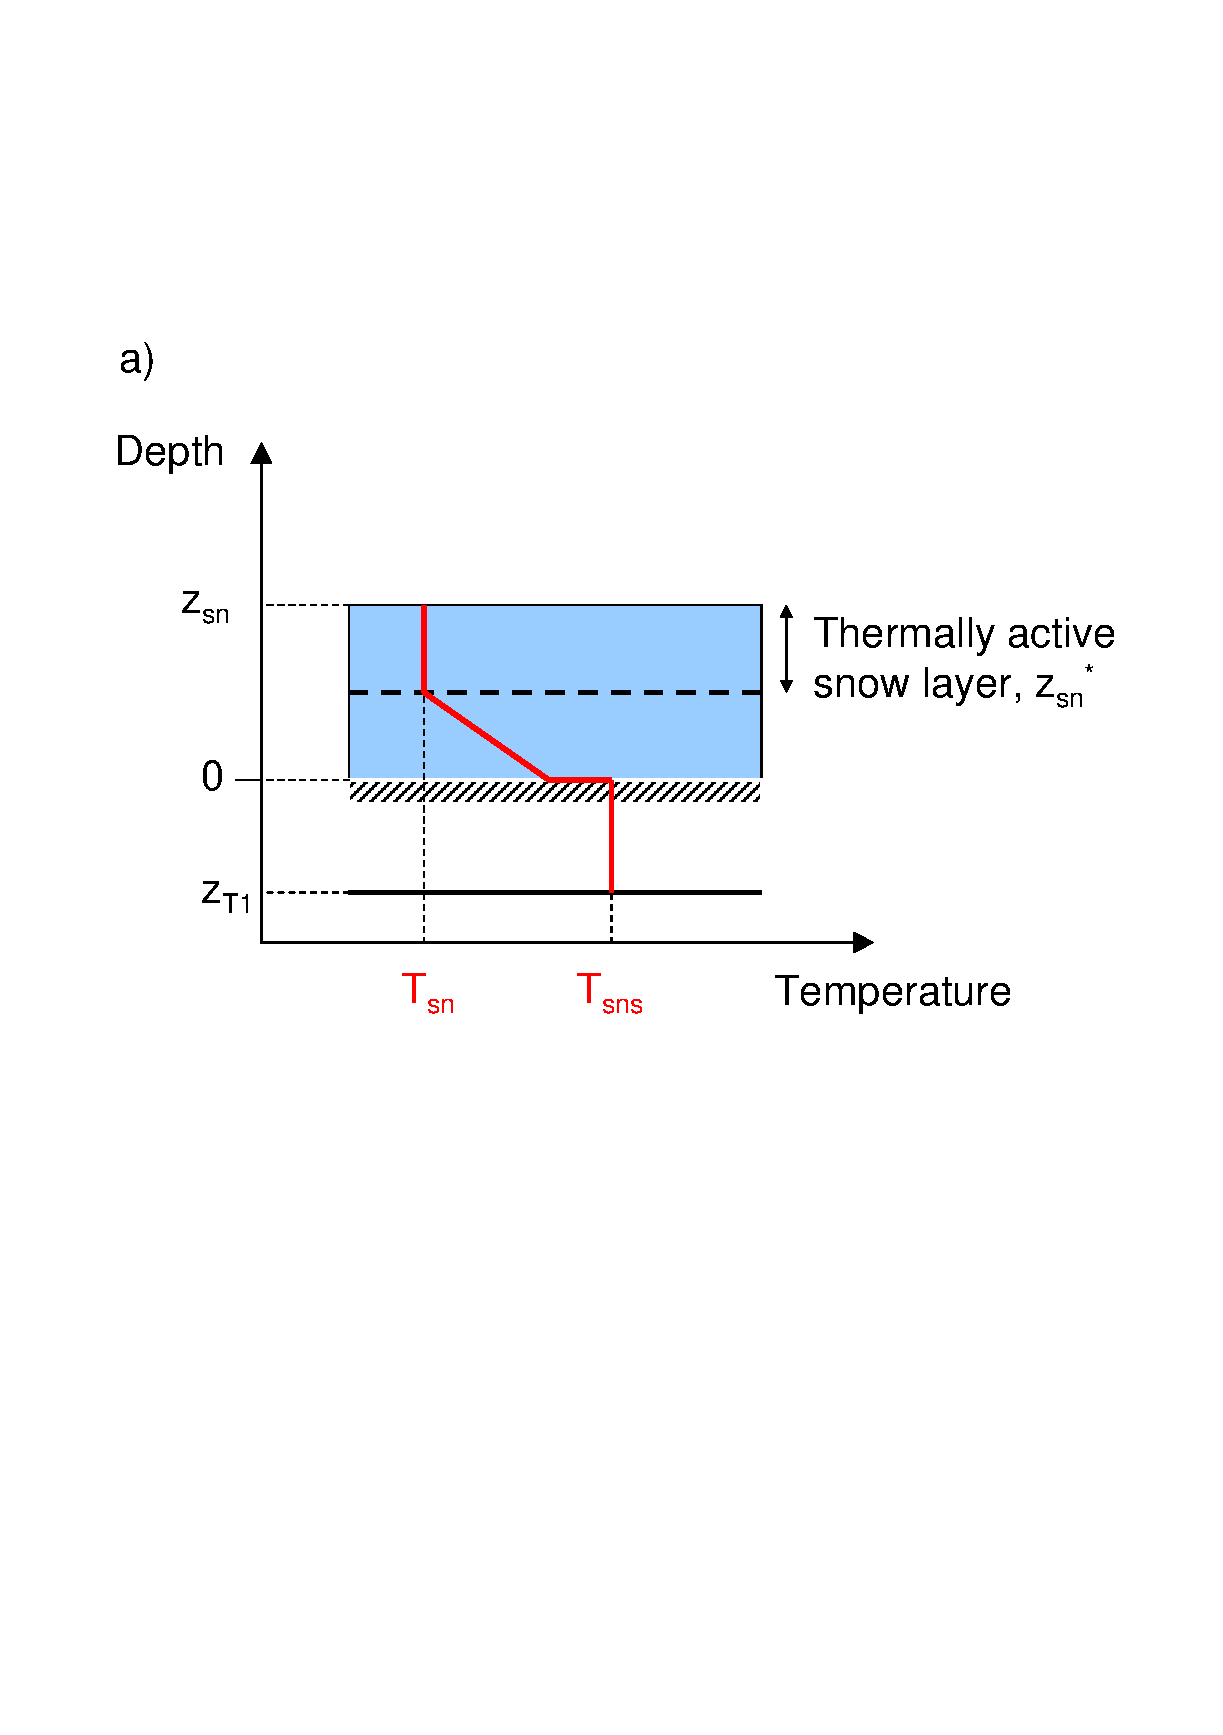
\includegraphics[width=8cm, trim=0 250 0 200]{figures/snow_layer_small_rn.eps}
 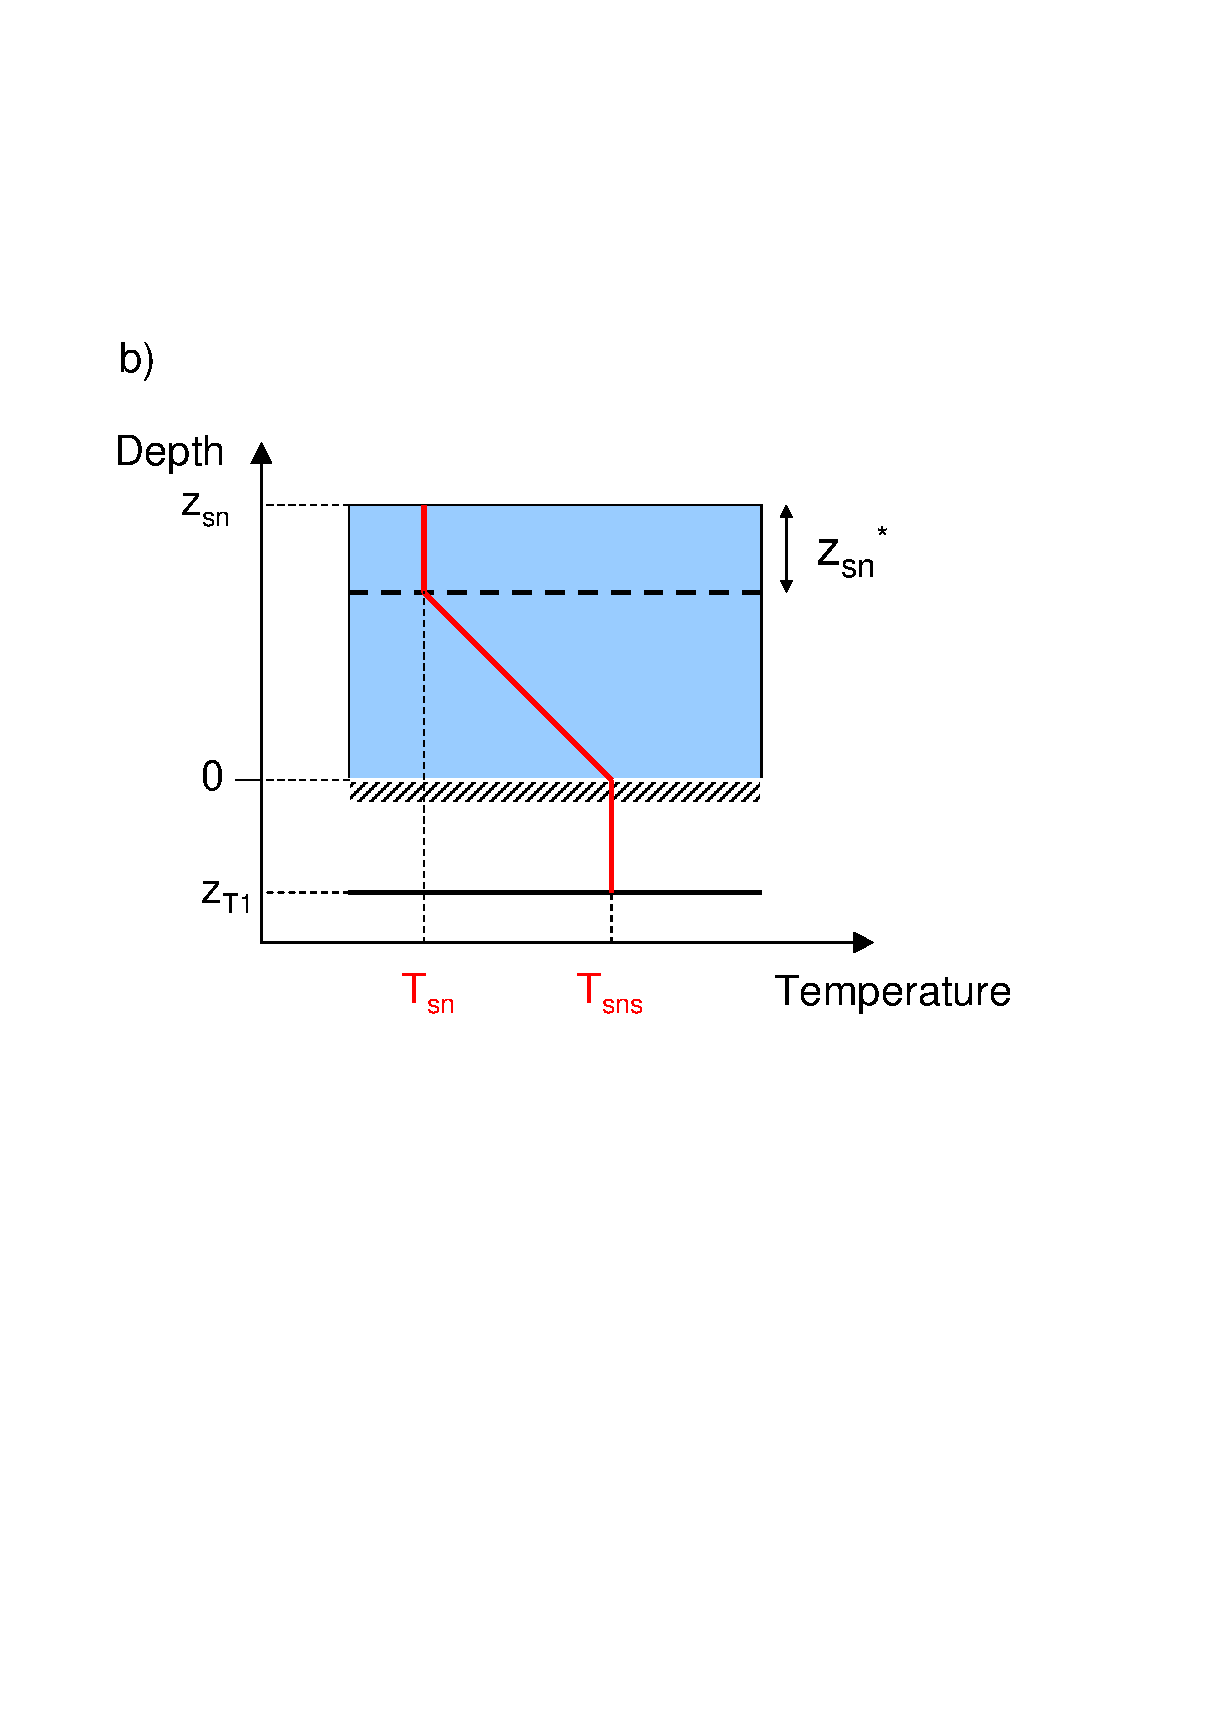
\includegraphics[width=8cm, trim=0 250 0 200]{figures/snow_layer_large_rn.eps}}
\caption{Principal sketch of the assumed temperature profile in a thin (a) and in a thick (b) snow
layer respectively.}
\label{snowtemp}
\end{figure}
%%%%%%%%%%%%%%%%%%%%%%%%%%%%%%%%%%%%%%

Figure \ref{snowtemp} shows the concept used describing the assumed temperature profile in the snow
for a thin and for a deep snow layer, respectively. The depth of the thermally active layer is defined
as $z_{sn}^* = \min(z_{sn},z_{snmax})$, where $z_{sn}$ is the actual snow depth and $z_{snmax}=0.15$m is the
maximum depth of the thermally active layer. The actual snow depth is defined as $z_{sn} = sn \rho_w/\rho_{sn}$,
where $\rho_{sn}$ and $\rho_w$ are the densities of snow and water, respectively. $\rho_{sn}$ is a prognostic
variable in the present LSS as described in Appendix \ref{sec:rhosn_albsn}.

The equation for the snow temperature is as follows:

%%%%%%%%%%%%%%%%%%%%%%%%
\begin{equation}
\del[T_{sn}]{t} = \Frac{1}{(\rho C)_{sn}  z_{sn}}\left[ \Phi_{sn} + \Lambda_{sn} (T_{sns} - T_{sn})\right],
\label{tsnow}
\end{equation}
%%%%%%%%%%%%%%%%%%%%%%%%

where $(\rho C)_{sn} = (\rho C)_{ice} \rho_{sn} / \rho_{ice}$ is the volumetric heat capacity of the snow and
$(\rho C)_{ice}$ is the volumetric heat capacity for ice. %($2.05 \cdot 10^6 \, J m^{-3} K^{-1}$ ),
$\Phi_{sn} = Rn_{sn} + H_{sn} + E_{sn}$ is the sum of the energy fluxes at the snow surface, net radiation and
sensible and latent heat fluxes, respectively, defined as

%%%%%%%%%%%%%%%%%%%%%%%%%
\begin{equation}
\label{eq:Rnsn}
Rn_{sn} = (1-\alpha_{sn})S\!\!\downarrow +\epsilon_{sn} (L\!\!\downarrow-\sigma T_{sn}^4),
\end{equation}
%%%%%%%%%%%%%%%%%%%%%%%%%

%%%%%%%%%%%%%%%%%%%%%%%%%
\begin{equation}
\label{eq:Hsn}
H_{sn} = \rho c_p \frac{T_{sn}-T_{am}}{r_{asn}},
\end{equation}
%%%%%%%%%%%%%%%%%%%%%%%%%

%%%%%%%%%%%%%%%%%%%%%%%%%
\begin{equation}
\label{eq:Esn}
E_{sn} = \rho L_e \frac{q_s(T_{sn})-q_{am}}{r_{asn}}.
\end{equation}
%%%%%%%%%%%%%%%%%%%%%%%%%

Note that these equations refer to the open land snow and must be replaced by the corresponding
forest equations in the case of forest snow. The snow albedo, $\alpha_{sn}$, is defined in Appendix \ref{sec:rhosn_albsn}.

The snow temperature in the layer below the thermally active layer is in principal unknown which means
that the heat transfer at the snow-soil interface is parameterised using a heat transfer
coefficient $\Lambda_{sn}$ between the snow and the underlying soil layer. Basically it is assumed that
the heat transfer at the snow-soil interface decreases with the depth of the snow layer.
$\Lambda_{sn}$ is simply a weighted average of the heat transfer coefficients of snow and soil, respectively, defined as

%%%%%%%%%%%%%%%%%%%%%%%%
\begin{equation}
\Lambda_{sn}^{-1} \, = \, 0.5 \, \Frac{z_{sn}}{\lambda_{sn}} + 0.5 \, \Frac{z_{T1}}{\lambda_{T}},
\label{lambdasn}
\end{equation}
%%%%%%%%%%%%%%%%%%%%%%%%

where $\lambda_{sn} = \lambda_{ice}( \rho_{sn}/\rho_{ice}) ^ {1.88}$ and
$\lambda_{T}$ is defined in Equation \ref{eq:lambdat} and $\lambda_{ice} = 2.2$ W m$^{-1}$ K$^{-1}$.

The snow temperature equation is part of a heat conduction problem including the soil temperature
equations. The resulting equation system is solved implicitly.
In the case of phase changes, i.e. melting of snow or freezing of liquid water in the snow, the time step is divided
into two parts, one where the temperature of the snow is kept constant and one where the snow temperature
is allowed to change.

\subsubsection{Phase changes in snow}

Two types of phase changes can take place in the snow pack; at positive energy balance
the snow temperature increases until the melting temperature is reached and melting starts,
while at negative energy balance any liquid water in the snow can partly refreeze at the same time as the
snow temperature drops. One can use different strategies to numerically solve this
phase-change problem. We have chosen to divide the time step into two parts which means that
upon melting, one part of the time step is used for increasing the temperature and the other part is
used to melt snow while keeping the snow temperature at the melting point. Upon freezing, one part of the
time step is used to freeze liquid water while keeping the snow temperature constant and the other part is
used to decrease the snow temperature.

%\subsection{Melting of snow}

The total energy per unit time available for the snow is

%%%%%%%%%%%%%%%%%%%%%%%%
\begin{equation}
\Phi_{tot} = \Phi_{sn} + \Lambda_{sn}(T_{sns} - T_{sn}).
\label{phitot}
\end{equation}
%%%%%%%%%%%%%%%%%%%%%%%%

If $\Phi_{tot} > 0$, we estimate the time, $\Delta t_{dtemp}$, it takes to bring $T_{sn}$ to $T_{melt}$ using Equation \ref{tsnow}.
If $\Delta t_{dtemp} \ge \Delta t$ the melting temperature is not reached and the snow temperature is calculated
using Equation \ref{tsnow} with $\Delta t_{dtemp} = \Delta t$. If $\Delta t_{dtemp} < \Delta t$  Equation \ref{tsnow} is used to
bring $T_{sn}$ to $T_{melt}$ and then $\Phi_{tot}$ is used during the rest of the time step,
$\Delta t_{dphase} = \Delta t - \Delta t_{dtemp}$, to melt snow while $T_{sn}$ is kept at the melting
temperature. The amount of melted snow, or water, becomes

%%%%%%%%%%%%%%%%%%%%%%%%
\begin{equation}
sn_{mel} =  \frac{\Delta t_{dphase} \Phi_{tot} }{ \rho_w L },
\label{snmel}
\end{equation}
%%%%%%%%%%%%%%%%%%%%%%%%

where $L$ is the latent heat of freezing.
This amount is used to increase the amount of liquid water kept in the snow, $w_{sn}$,
until it reaches a maximum allowed amount, $w_{snsat}=\Delta_{snsat} sn$, where $\Delta_{snsat}$ is
set to 10\%. Any excess liquid water goes to the soil.

%\subsection{Freezing of liquid water in snow}

At negative energy balance for the snow, i.e. $\Phi_{tot} < 0$, the snow temperature should drop
but if the liquid water content is non-zero we should also freeze some of the water.
In contrast to the straight forward melting processes the parameterisation of the freezing process
is not as obvious in the case of $w_{sn}>0$. How much of the liquid water that should be frozen during a
certain time does, in principle, depend on where the water is located in the snow layer and how the
characteristics of the heat transfer in the snow looks like. With a snow model as simple as the one
described here it is impossible to make any physically valid estimation on this amount. Thus,
we are let out to some estimation based on assumptions. The assumptions made here are based on the fact that snow melt
mainly occurs at the top of the snow layer and that the melt water is located where melting occurs.
The larger the amount of melt water in the snow the deeper it penetrates. We estimate a fraction,
$\Delta_{freeze}$, of the liquid water amount that is allowed to freeze according to

%%%%%%%%%%%%%%%%%%%%%
\begin{equation}
\Delta_{freeze} = \min\left( \frac{sn_{freeze} \rho_{sn}}{\rho_w} \frac{\Delta_{snsat}}{w_{sn}}, 1 \right),
\label{dfreeze}
\end{equation}
%%%%%%%%%%%%%%%%%%%%%

where $sn_{freeze}$ is an assumed depth of snow over which freezing is allowed to be active, set to $0.03$ m.
In other words, the equivalent water amount corresponding to $sn_{freeze}$ is $sn_{freeze} \rho_{sn}/\rho_w$.
The corresponding maximum liquid water amount allowed is given by $sn_{freeze} \rho_{sn}/\rho_w \Delta_{snsat}$
which is related to the actual liquid water amount, $w_{sn}$.
The value of $sn_{freeze}$ must be estimated by trial and error examining the simulated snow
temperature against observations.
$\Delta_{freeze}$ is used to calculate the fraction of the time step to be used for freezing of water,
$\Delta t_{dphase} = \Delta_{freeze} \Delta t$. During this time the snow temperature is kept constant.
Cooling of the snow temperature takes place during the rest of the time step, $\Delta t_{dtemp} = \Delta t - \Delta t_{dphase}$,
by applying Equation \ref{tsnow}.
If the available water is less than the corresponding water given by $\Delta t_{dphase}$, the time for freezing
of water is reduced.

The change in open-land snow water equivalent is as follows:

%%%%%%%%%%%%%%%%%%%%%
\begin{equation}
sn^{\tau+1}=sn^{\tau}+\frac{\Delta t}{\rho_w}\left[ A_{sn}(F+P_{sn-}) +A_{opl}(F+P_{opl-}-F_{opl+}) + A_{sn} \frac{E_{sn}}{L_e} \right] - sn_{mel},
\label{dsnst}
\end{equation}
%%%%%%%%%%%%%%%%%%%%%

which includes the three phase changes $P_{sn-}$, rain freezing on cold snow, $P_{opl-}$, rain freezing on cold ground and $F_{opl+}$,
snow melting on warm ground. $F$ denotes snowfall (kg m$^{-2}$s$^{-1}$).
The change in forest snow water equivalent is given by a corresponding equation.


%%%%%%%%%%%%%%%%%%%%%%%%%%%%%%%%%%%%%%%%%%%%%%%%%%%%%%%%%%%%%%%%%%%%%%%%%%%%%%%%%%%%%%%%%%%%%
%%%%%%%%%%%%%%%%%%%%%%%%%%%%%%%%%%%%%%%%%%%%%%%%%%%%%%%%%%%%%%%%%%%%%%%%%%%%%%%%%%%%%%%%%%%%%

\subsection{Soil processes}
\label{sec:soiltemp}

The soil is characterized by its texture and water content. The scheme uses twelve different
texture classes based on the percentage of clay and sand in the texture triangle according to \cite{kn:Hillel80} (see Table \ref{textureclasses}).
The hydraulic properties for each soil type are based on \cite{kn:Clapp78} and \cite{kn:McCumber81} and are specified in
terms of total porosity $\theta_{sat}$ (m$^{3}$m$^{-3}$), field capacity $\theta_{fc}$ (m$^{3}$m$^{-3}$),
wilting point $\theta_{wi}$ (m$^{3}$m$^{-3}$),
matric potential at saturation $\psi_{sat}$ (m),
hydraulic conductivity at saturation $\gamma_{sat}$ (m s$^{-1}$), Clapp and Hornberger soil parameter $b$, and
amount of quartz $cq$ (-).

%%%%%%%%%%%%%%%%%%%%%%%%%%%%%%%%%%%%%%%%%%%%%%%%%%%%%%%%%%%%%%%%%%%%%%%%%%%%%%%%%%%%%%%%%%%%%
%%%%%%%%%%%%%%%%%%%%%%%%%%%%%%%%%%%%%%%%%%%%%%%%%%%%%%%%%%%%%%%%%%%%%%%%%%%%%%%%%%%%%%%%%%%%%

\subsubsection{Soil temperature}

The soil heat transfer equation applied for each soil layer can be written as

%%%%%%%%%%%%%%%%%%%%%%%%%
\begin{equation}
  \label{eq:dTsdt}
  [(\rho C)_{s\theta} + \Delta C_{fs}] \del[T_s]{t} = \del[]{z} \left( \phi^{t,b} + \lambda_T \del[T_s]{z} \right).
\end{equation}
%%%%%%%%%%%%%%%%%%%%%%%%%

Here $(\rho C)_{s\theta}$ is the volumetric wet soil heat capacity for a soil moisture content of $\theta$
(m$^{3}$m$^{-3}$) defined as $(\rho C)_{sw} = (\rho C)_s + \theta \rho_w C_w$.

Definition of $(\rho C)_s$XXX??

The present LSS does not include the solid phase of soil water which means that e.g. the thermal process
related to the latent heat of fusion/freezing is absent. This process is important since
it acts to delay the soil cooling in autumn and the soil warming in spring. To simulate this effect
we apply a modification of the soil heat capacity, $\Delta C_{fs}$, as suggested by
\cite{kn:Viterbo99}, which increases the total soil heat capacity in the temperature range -3 to +1\deg C.

The heat conductivity $\lambda_T$ depends on the soil water content as described by \cite{kn:McCumber81}

%%%%%%%%%%%%%%%%%%%%%%%%%
\begin{equation}
\lambda_T(\theta) = - a \psi_{sat}^{-1/\log10} \left( \frac{\theta_{sat}}{\theta} \right)^{-b/\log10}.
\label{eq:lambdat}
\end{equation}
%%%%%%%%%%%%%%%%%%%%%%%%%

Here $a$ is an empirical soil thermal conductivity parameter.

The top boundary condition, $\phi^t$, is represented by the total flux at the surface, $\phi_{fors}$ or $\phi_{opls}$
in the cases of forest soil or open-land soil, respectively, or the heat transfer at the soil/snow interface
in the cases of snow covered soil in the forest or at the open land as defined in Section \ref{sec:snow}.
At the bottom a zero-flux condition is assumed, i.e. $\phi^b=0$.

Since there are four different top boundary conditions for the soil we will have four soil columns with
different evolutions of their soil temperature profiles. The soil is divided into five layers in the vertical
with respect to temperature which thus results in 20 prognostic soil temperatures.
If the fractional snow cover changes during a time step the soil temperatures have to be adjusted accordingly to
avoid an artificial change of the total heat content of the soil.

%%%%%%%%%%%%%%%%%%%%%%%%%%%%%%%%%%%%%%%%%%%%%%%%%%%%%%%%%%%%%%%%%%%%%%%%%%%%%%%%%%%%%%%%%%%%%
%%%%%%%%%%%%%%%%%%%%%%%%%%%%%%%%%%%%%%%%%%%%%%%%%%%%%%%%%%%%%%%%%%%%%%%%%%%%%%%%%%%%%%%%%%%%%

\subsubsection{Soil moisture, drainage and runoff}
\label{sec:soilmoist}

The vertical transport of water in the unsaturated soil is usually expressed using Richards equation
\cite[]{kn:Hillel80}

%%%%%%%%%%%%%%%%%%%%%%%%%
\begin{equation}
\label{eq:theta}
\del[\theta]{t} = \del[]{z}\left( \lambda \del[\theta]{z} \right) - \del[\gamma]{z} + S(\theta,z),
\end{equation}
%%%%%%%%%%%%%%%%%%%%%%%%%

where $\lambda$ is the hydraulic diffusivity (m$^2$s$^{-1}$), $\gamma$ is the hydraulic conductivity
(ms$^{-1}$), and $S(\theta,z)$ is a volumetric source/sink term (m$^3$m$^{-3}$s$^{-1}$).
The hydraulic
diffusivity is parameterized according to \cite{kn:McCumber81}

%%%%%%%%%%%%%%%%%%%%%%%%%
\begin{equation}
\label{eq:lambda}
\lambda = \frac{b \gamma_{sat} (-\psi_{sat})}{\theta_{sat}} \left( \frac{\theta}{\theta_{sat}} \right)^{b+2}.
\end{equation}
%%%%%%%%%%%%%%%%%%%%%%%%%

The volumetric source/sink term generally includes effects of precipitation, runoff, root extraction, and
phase changes of ice to liquid water. However, as described above we do not explicitly include any phase
changes of ice to liquid water in the soil but instead we parameterize the effect that soil ice would have had
on soil heat capacity and root extraction.
In the present LSS we replace the hydraulic conductivity term, $\delt[\gamma]{z}$, in Equation \ref{eq:theta} with
a drainage/runoff parameterization as part of the $S(\theta,z)$ term. The final sources and sinks in $S(\theta,z)$
then become;
supply of water at the soil surface, $S^w(z_0)$, evaporation/condensation at the soil surface, $S^e(\theta,z_0)$,
loss due to root extraction, $S^{re}(\theta,z_d)$, and drainage/runoff, $S^{dr}(\theta,z_d)$, at each soil
layer/interface $z_d$. 
No lateral transport of water exists in the scheme.
%Surface runoff is often included in soil water schemes, however,
%we argue that surface runoff has no physical ground on scales on which this scheme operates, i.e. on horizontal scales
%of tenth of kilometers. Therefore surface runoff does not occur in the present LSS.
The supply of water at the soil surface is represented by contributions from rainfall,
snow-melt water, and throughfall from vegetation. The evaporation/condensation at the soil surface is
represented by two terms; one for the forest floor soil, which is the $E_{fors}$ equation in Equation
array \ref{eq:forarray}, and one for the open land soil, Equation \ref{eq:Eopls}.

The loss due to root extraction is given by the transpiration parts of Equations \ref{eq:forarray}($E_{forc}$) and \ref{eq:Eoplv}, i.e.
with the transpiration components of the Halstead coefficients, $h_{vfor}^{tr}$ and $h_{vopl}^{tr}$.

The drainage/runoff parameterization is based on the
so called $\beta$-formulation as used in the hydrological HBV model \cite[]{kn:Lindstrom97}. The drainage can then
be written as a source/sink term

%%%%%%%%%%%%%%%%%%%%%%%%%
\begin{equation}
\label{eq:Sdr}
S^{dr}(\theta,z_n) = S^{dr}(\theta,z_{n-1}) \left( \frac{\theta - \theta_{wi}}{\theta_{fc} - \theta_{wi}} \right)^\beta, 
\end{equation}
%%%%%%%%%%%%%%%%%%%%%%%%%

where the upper boundary condition $S^{dr}(\theta,z_0)=S^w(z_0)$ and the resulting runoff is given
by $S^{dr}(\theta,z_2)$. 
The exponent $\beta$ set to zero would imply a grid square with no water holding
capacity at all while a high $\beta$ value indicates such homogeneous conditions that the whole
grid square may be regarded as a bucket that overflows when its field capacity is reached. $\beta$ is
thus more an index of heterogeneity than of soil property.
$\beta$is a tuning parameter and in the present model we use $\beta=2$, which the same value as is used in
the HBV model \cite[]{kn:Bergstrom98}. 

There are three prognosic layers of soil moisture. The thicknesses of the top and second layers are constant
(Figure \ref{lssfig}) while the thickness of the third layer is given by the root depth according to ECOCLIMAP.
There are also separte soil water columns under forst and open land, respectively. Thus, in total we have
six prognostic soil water variables $\theta$.

See Appendix \ref{sec:solvingsoilmoisture} for details on soil moisture.


%%%%%%%%%%%%%%%%%%%%%%%%%%%%%%%%%%%%%%%%%%%%%%%%%%%%%%%%%%%%%%%%%%%%%%%%%%%%%%%%%%%%%%%%%%%%%
%%%%%%%%%%%%%%%%%%%%%%%%%%%%%%%%%%%%%%%%%%%%%%%%%%%%%%%%%%%%%%%%%%%%%%%%%%%%%%%%%%%%%%%%%%%%%

\section{Physiography}
\label{sec:physiography}

\subsection{Orography}

\subsection{Land-use physiography}

The land-use physiography in RCA is based on ECOCLIMAP \cite[]{}.
The data and source code is according to ``october 04, corrected september 2006'' as indicated on the web-page \cite[]{}.
In addition to the ECOCLIMAP data we utilize information on soil carbon \cite[]{}.

\verb+http://www.cnrm.meteo.fr/gmme/PROJETS/ECOCLIMAP/page_ecoclimap.htm+

For RCA purposes we have modified the ECOCLIMAP source code:
\begin{itemize}
\item Redefined the specifications of \verb+NTILE=3+ in \verb+vegtype_to_patch.f90+
\item Added output of \verb+F_lake+ in \verb+ecoclimap_parameters.f90+
\item Added reading and processing of soil carbon in \verb+ecoclimap_parameters.f90+
\end{itemize}

The three tiles are defined as: 

%%%%%%%%%%%%%%%%%%%%%%%%%%%%%%
\begin{table}[h]
\caption{The three land tiles in RCA}
\begin{center}
\begin{footnotesize}
\begin{tabular}{lll}
\hline
Tile	& Description			& ECOCLIMAP IVEGTYPE \\
\hline
\hline
t01	& open land low vegetation	&  \verb+NVT_(all_no_tree)+		\\
t02	& coniferous forest		& \verb+NVT_CONI+			\\
t03	& broadleaf forest		& \verb+NVT_TREE+ or \verb+NVT_EVER+	\\
\hline
\end{tabular}
\end{footnotesize}
\end{center}
\label{RCAtiles}
\end{table}
%%%%%%%%%%%%%%%%%%%%%%%%%%%%%%%%%%%%

The available ECOCLIMAP parameters in RCA are listed in Appendix \ref{sec:ECOCLIMAPspecifications}.


\subsubsection{Root distribution}
\label{sec:rootdistribution}

The root depths for open land and forest, respectively, are specified using the ECOCLIMAP parameters
\verb+droot_t1+, \verb+droot_t2+ and \verb+droot_t3+:

%%%%%%%%%%%%%%%%
\begin{equation}
\begin{array}{l}
D_{root\_opl} = \max(droot\_t1,0.332),		\\
D_{root\_for} = \max(droot\_t2,droot_t3,1.5).	\\
\end{array}
\end{equation}
%%%%%%%%%%%%%%%%

The vertical distribution of roots is parametersiaed following \cite{kn:Jackson96}.
The extinction coefficient $\beta_{root}$ represents how the roots are distributed.
High $\beta_{root}$-values correspond to a greater proportion of roots at depths.
We calculate $\beta_{root}$ assuming that 99\% ($Fr_{root}=0.99$) of the roots
occopy the root depth $D_{root}$:

%%%%%%%%%%%%%%%%
\begin{equation}
\beta_{root} = (1-Fr_{root})^{\frac{1}{D_{root}}}.
\end{equation}
%%%%%%%%%%%%%%%%

The $\beta_{root}$-values are maximized to 0.975.
Using $\beta_{root}$ we can calculate the fraction of roots in each soil layer

%%%%%%%%%%%%%%%%
\begin{equation}
Fr_{root\_n} = (1-\beta_{root\_n})^{z_{\theta n}},
\end{equation}
%%%%%%%%%%%%%%%%

which is used in the calculation of the vegetation surface resistance.
According to \cite{kn:Canadell96} plants have the ability to compensate for dry condtions at a certain root
level by increasing the efficiency of water uptake at other levels. This effect is accounted
for as

%%%%%%%%%%%%%%%%
\begin{equation}
\left\{
\begin{array}{r l}
Fr_{root\_n}=		& SWA_n Fr_{root\_n}, \\
Fr_{root\_{n+1}}=	& Fr_{root\_{n+1}} + (1 - SWA_n) Fr_{root\_n} ), \\
\end{array}
\right.
\end{equation}
%%%%%%%%%%%%%%%%

where $n$ represents soil layers 1 and 2 and $SWA$ is the soil-water availability defined as

%%%%%%%%%%%%%%%%
\begin{equation}
SWA = \frac{\theta - \theta_{wi}}{\theta_{fc} - \theta_{wi}}.
\end{equation}
%%%%%%%%%%%%%%%%


\subsection{Lake-depth database}

\bigskip

{\bf Acknowledgments:} 

The authors are grateful for discussions with colleagues at Rossby Centre, SMHI, who gave valuable input to this report.
The development of the LSS and the implementataion of FLake have been supported by a number of projects:
SWECIA, RESM, ADSIMNOR, MERGE, CLARIS LPB, Visby programmme,... 


\newpage
\appendix

\section{Aerodynamic resistances within the forest}
\label{sec:rafor}

The parameterisation of the bulk aerodynamic resistance $r_b= 1/g_b$ is based on \cite{kn:Choudhury88},
where the conductance between the canopy and the canopy air, $g_b$, is defined as

%%%%%%%%%%%%%%%%%%%%%%%%%
\begin{equation}
  \label{eq:condrb}
  g_b = \frac{2 LAI a}{\alpha'}\left(\frac{u_{for}}{lw}\right)^{1/2}[1-\exp(-\alpha'/2)].
\end{equation}
%%%%%%%%%%%%%%%%%%%%%%%%%

The conductance is modified with a free convection correction according to \cite{kn:Sellers86}

%%%%%%%%%%%%%%%%%%%%%%%%%
\begin{equation}
  \label{eq:freeconv}
  g_b = g_b + \frac{LAI}{890} \left(\frac{T_{forc} - T_{fora}}{lw}\right)^{1/4}.
\end{equation}
%%%%%%%%%%%%%%%%%%%%%%%%%

The aerodynamic resistance $r_d$ is based on \cite{kn:Choudhury88}

%%%%%%%%%%%%%%%%%%%%%%%%%
\begin{equation}
  \label{eq:rd}
  r_d = \frac{z_{for}\exp(\alpha)}{\alpha K(z_{for})} [\exp(-\alpha z_0'/z_{for}) - \exp(-\alpha(d + z_0)/z_{for})],
\end{equation}
%%%%%%%%%%%%%%%%%%%%%%%%%

\noindent where

%%%%%%%%%%%%%%%%%%%%%%%%%
\begin{equation}
  \label{eq:Kh}
  K(z_{for} ) = k (z_{for} - d) u_{*for} = \frac{k^2 (z_{for} - d) u}{\ln\frac{z_{for} - d}{z_0}}.
\end{equation}
%%%%%%%%%%%%%%%%%%%%%%%%%

The displacement height is defined as \cite[]{kn:Choudhury88}:

%%%%%%%%%%%%%%%%%%%%%%%%%
\begin{equation}
  \label{eq:disph}
  d = 1.1 z_{for} \ln[1 + (c_d LAI_f)^{1/4}]
\end{equation}
%%%%%%%%%%%%%%%%%%%%%%%%%

\noindent where the leaf drag coefficient $c_d$ is defined as \cite[]{kn:Sellers96}:

%%%%%%%%%%%%%%%%%%%%%%%%%
\begin{equation}
  \label{eq:cd}
  c_d = 1.328 \left[\frac{2}{\mathrm{Re}^{1/2}}\right] + 0.45 \left[ \frac{1}{\pi}(1-\chi_L) \right]^{1.6}
\end{equation}
%%%%%%%%%%%%%%%%%%%%%%%%%

\noindent where $\chi_L$ is the Ross-Goudriaan leaf angle distribution function, which has
been estimated according to \cite{kn:Monteith75} (see Table \ref{independent}), and
Re is the Reynolds number defined as

%%%%%%%%%%%%%%%%%%%%%%%%%
\begin{equation}
  \label{eq:Re}
  \mathrm{Re} = \frac{u_l lw}{\upsilon}.
\end{equation}
%%%%%%%%%%%%%%%%%%%%%%%%%

The unstable transfer correction for $r_d=r_d/\psi_H$ according to \cite{kn:Sellers86},
where

%%%%%%%%%%%%%%%%%%%%%%%%%
\begin{equation}
  \label{eq:phih}
  \psi_H = \left[ 1 + 9 \frac{T_{fors} - T_{fora}}{T_{fors} u_{for}^2} z_{for} \right]^{1/2}.
\end{equation}
%%%%%%%%%%%%%%%%%%%%%%%%%

For the estimations of $r_b$ and $r_d$ the friction velocity at the forest tile, $u_{*for}$, is needed as
well as the wind speed at the top of the forest, i.e. $u_{for}$ at $z_{for}$. $u_{*for}$ is estimated
from the drag coefficient of momentum calculated as in Equation \ref{eq:Ch} but with $z_{0h}$ replaced by
$z_{0m}$. $u_{for}$ is then reached in two steps: firstly the wind speed $u_{trans}$ at a transition level $z_{trans}$,
located between $z_{am}$ and $z_{for}$, is calculated as

%%%%%%%%%%%%%%%%%%%%%%%%%
\begin{equation}
  \label{eq:utrans}
u(z_{trans}) = \frac{u_{*for}}{k} \left[ \ln\frac{z_{trans}-d}{z_{0m}} - \Psi_m\left( \frac{z_{trans}-d}{L} \right) \right],
\end{equation}
%%%%%%%%%%%%%%%%%%%%%%%%%

where $z_{trans}$ is defined as

%%%%%%%%%%%%%%%%%%%%%%%%%
\begin{equation}
  \label{eq:translev}
  z_{trans} = z_{for} + 11.785 z_{0m}.
\end{equation}
%%%%%%%%%%%%%%%%%%%%%%%%%

Secondly, $u_{for}=u(z_{trans}) - G_2 \Delta u(z_{trans},z_{for})$, where $\Delta u(z_{trans},z_{for})=
u(z_{trans})-u(z_{for})$ and $G_2$ is an adjustment factor which is equal to 0.75 according to
\cite{kn:Xue91}.


%%%%%%%%%%%%%%%%%%%%%%%%%%%%%%
\begin{table}[h]
\caption{Surface independent parameters}
\begin{center}
\begin{footnotesize}
\begin{tabular}{clllll}
\hline
Symbol		& Definition			& Unit		& Value	& Reference		& Comment \\
\hline
\hline
$g$		& Acceleration of gravity	& m s$^{-2}$	& 9.81	\\
$G_2$		& Adjustment factor		& -		& 0.75	& \cite{kn:Xue91}	& Eq. 13 \\
$k$		& von Karman constant		& -		& 0.4 \\
$a$		& 				& m s$^{-1/2}$	& 0.01	& \cite{kn:Choudhury88}	& Eq. 26 \\
$\alpha'$	& attenuation coeff. for wind	& -		& 3	& \cite{kn:Choudhury88} & p 386 \\
$lw$		& leaf width			& m		& 0.02	\\
$\alpha$	& attenuation coeff. for mom.	& -		& 2	& \cite{kn:Choudhury88} & p 386 \\
$z_0'$		& roughness of soil surface	& m		& 0.007	\\
$\chi_L$	& Ross-Goudriaan leaf angle dist. & -		& 0.12	& \cite{kn:Monteith75}	& p 26 \\
$u_l$		& Typical local wind speed	& \ms		& 1	& \cite{kn:Sellers96}	& Eq. B7 \\
$\upsilon$	& Kinematic viscos. of air	& m$^2$ s$^{-1}$ & $0.15\cdot 10^{-4}$ \\

\hline
\end{tabular}
\end{footnotesize}
\end{center}
\label{independent}
\end{table}
%%%%%%%%%%%%%%%%%%%%%%%%%%%%%%%%%%%%


%%%%%%%%%%%%%%%%%%%%%%%%%%%%%%%%%%%%%%%%%%%%%%%%%%%%%%%%%%%%%%%%%%%%%%%%%%%%%%%%%%%%%%%%%%%%%%%%%%%%%%%%%%%

\section{Snow density and snow albedo}
\label{sec:rhosn_albsn}

\subsection{Snow density} 

The density of the snow increases exponentially with time towards a maximum value as long as no fresh snow is
added by snowfall. The total density of the snow pack is a weighted value of the dry snow and of the liquid water
content. Assuming that we have the density of the dry snow calculated, $\rho_{snd}$, which compare to the
water equivalent of the dry snow, $sn_d$, we can combine that
with any snowfall, $F$, during the time step to a temporary new dry snow density

%%%%%%%%%%%%%%%%%%%%%%%%%
\begin{equation}
\rho_{snd}^*=\Frac{sn_d^{\tau} \rho_{snd}^{\tau} + (\Delta t F /\rho_w) \rho_{snmin}}{sn_d^{\tau} + (\Delta t F/\rho_w)},
\label{rhost}
\end{equation}
%%%%%%%%%%%%%%%%%%%%%%%%%

where $\rho_{snmin}=100$ kg m$^{-3}$ is the minimum density of dry snow. The new value of the dry snow
density becomes

%%%%%%%%%%%%%%%%%%%%%%%%%
\begin{equation}
\rho_{snd}^{\tau + 1}= (\rho_{snd}^* - \rho_{snmax}) \exp(- \tau_f  \Delta t/\tau_1 ) + \rho_{snmax},
\label{rhosnd}
\end{equation}
%%%%%%%%%%%%%%%%%%%%%%%%%

where $\rho_{snmax}=300$ kg m$^{-3}$ is the maximum density of dry snow. The time scales
$\tau_1=86400$ s and $\tau_f=0.24$ give an e-folding time of about 4 days. Combining the
new dry snow density with the liquid water content in the snow gives the total density of the snow

%%%%%%%%%%%%%%%%%%%%%%%%%
\begin{equation}
\rho_{sn}^{\tau + 1}= \Delta_{snd}^{\tau + 1} \rho_{snd}^{\tau + 1} + (1 - \Delta_{snd}^{\tau + 1})\rho_w,
\label{rhosn}
\end{equation}
%%%%%%%%%%%%%%%%%%%%%%%%%

where $\Delta_{snd}$ is the fraction of dry snow to total snow, i.e. $\Delta_{snd}=(sn - w_{sn})/sn$.

\subsection{Snow albedo} 
\label{sec:snowalb}

The net radiation balance at the surface for open land snow is given by
$Rn_{sn} = (1-\alpha_{sn})S\!\!\downarrow +\epsilon_{sn} (L\!\!\downarrow-\sigma T_{sn}^4)$,
where the snow albedo, $\alpha_{sn}$, for open-land snow is a prognostic variable.
The albedo for snow in the forest is set constant to $0.5$.

The parameterisation of snow albedo evolution is divided into three main cases;
snow fall situations, melting conditions and the rest (no snow fall and no melting).
In the case of snow fall we distingusih between melting and non-melting conditions.

\begin{itemize}
\item For snow-fall events (snow fall intensity exceeds 0 kg m$^{-2}$ s$^{-1}$)
   \begin{itemize}
   \item and melting conditions ($sn_{mel}>0$)
%%%%%%%%%%%%%%%%%%%%%%%%%
\begin{equation}
\left\{
\begin{array}{r l}
\alpha_{sn}^{*}		=	& \left( \frac{F_{sn} f_{sn2am} }{A_{opl} + A_{sn}} \right)^{f_{frsn}}  \\
\alpha_{sn}^{\tau+1}	=	& \alpha_{sn}^\tau (1 - \alpha_{sn}^{*} ) + \alpha_{sn,melt} \alpha_{sn}^{*} \\
\end{array}
\right.
\end{equation}
%%%%%%%%%%%%%%%%%%%%%%%%%

   \item and non-melting conditions ($sn_{mel}=0$)
%%%%%%%%%%%%%%%%%%%%%%%%%
\begin{equation}
\left\{
\begin{array}{r l}
\alpha_{sn}^{*}		=	& \left( \frac{F_{sn} f_{sn2af} }{A_{opl} + A_{sn}} \right)^{f_{frsn}}  \\
\alpha_{sn}^{\tau+1}	=	& \min\left[ \alpha_{sn,max} , \alpha_{sn}^\tau (1 - \alpha_{sn}^{*} ) + \alpha_{sn,freeze} \alpha_{sn}^{*} \right] \\
\end{array}
\right.
\end{equation}
%%%%%%%%%%%%%%%%%%%%%%%%%

  \end{itemize}

\item For conditions with no snow fall but melting ($sn_{mel}>0$)
%%%%%%%%%%%%%%%%%%%%%%%%%
\begin{equation}
\left\{
\begin{array}{r l}
\alpha_{sn}^{*}	=		& \max\left\{ \alpha_{sn,melt} , \alpha_{sn}^\tau - \left[ (\alpha_{sn,max}-\alpha_{sn,melt})  \frac{sn_{mel}}{f_{albdec}*(A_{opl} + A_{sn})} \right]  \right\}  \\
\alpha_{sn}^{\tau+1}	=		& \min\left[ \alpha_{sn}^{*} , (\alpha_{sn}^\tau - \alpha_{sn,min} ) \exp(-\tau_{fsn} \frac{\Delta t}{\tau_{1sn}}) + \alpha_{sn,min} \right] \\
\end{array}
\right.
\end{equation}
%%%%%%%%%%%%%%%%%%%%%%%%%

\item For conditions with no snow fall and no melting
%%%%%%%%%%%%%%%%%%%%%%%%%
\begin{equation}
\alpha_{sn}^{\tau+1} = \alpha_{sn}^\tau - \frac{ \tau_{asn} \Delta t}{ \tau_{1sn} (1+ 0.01 (T_{sn}-T_{melt})^4) }
\label{rhosn}
\end{equation}
%%%%%%%%%%%%%%%%%%%%%%%%%

\end{itemize}

where

%%%%%%%%%%%%%%%%%%%%%%%%%
\begin{equation}
\left\{
\begin{array}{r l}
f_{sn2am} = 1000  \Frac{\alpha_{sn,max} - \alpha_{sn,min}} {\rho_{sn,min} Z_{sn,\alpha_{sn,max}} (\alpha_{sn,melt}   - \alpha_{sn,min})} \\
f_{sn2af} = 1000  \Frac{\alpha_{sn,max} - \alpha_{sn,min}} {\rho_{sn,min} Z_{sn,\alpha_{sn,max}} (\alpha_{sn,target} - \alpha_{sn,min})} \\
\end{array}
\right.
\end{equation}
%%%%%%%%%%%%%%%%%%%%%%%%%

and

\begin{description}
\item[$\alpha_{sn,target}$  =]  0.9 is a target albedo for resetting snow albedo at snow fall events 
\item[$Z_{sn,\alpha_{sn,max}}$ =]  0.05 is the snowlayer depth that resets albedo to maximum its value
\item[zalbareap =]  0.8  is a scaling factor for fraction covered by fresh snow
\item[$\alpha_{sn,melt}$  =]  0.7 is the maximum snow albedo at melting conditions.
\item[zalbmelts =]  0.003  get a decay to zalbmelt from albsnmax with 0.003 m of snowmelt
\item[zexpalb   =] exp(-taufsn*dtime/tau1sn)
\end{description}




%%%%%%%%%%%%%%%%%%%%%%%%%%%%%%%%%%%%%%%%%%%%%%%%%%%%%%%%%%%%%%%%%%%%%%%%%%%%%%%%%%%%%%%%%%%%%%

\section{Diagnostic quantities}
\label{sec:diagnostics}


Except for prognostic variables at the surface and at atmospheric model levels there is a need to calculate diagnostic
variables that correspond to common observed quantities. Some of the most important diagnostic variables are air temperature and
specific humidity at 2m height ($T2m$ and $q2m$) and wind speed components at 10m height ($u10$ and $v10$).
The calculation of these diagnostic variables for a given height $z$ are based on Monin-Obukhov similarity theory: 

%%%%%%%%%%%%%%%%
\begin{equation}
\left\{
\begin{array}{l}
u(z) = \frac{u_*}{k} \left[ \ln\frac{z}{z_{0m}} - \Psi_m\left( \frac{z}{L} \right) \right] \\
v(z) = \frac{v_*}{k} \left[ \ln\frac{z}{z_{0m}} - \Psi_m\left( \frac{z}{L} \right) \right] \\
T(z) = T_s + \frac{\theta_*}{k} \left[ \ln\frac{z}{z_{0h}} - \Psi_h\left( \frac{z}{L} \right) \right] \\
q(z) = q_s + \frac{q_*}{k} \left[ \ln\frac{z}{z_{0q}} - \Psi_q\left( \frac{z}{L} \right) \right] \\
\end{array}
\right.
\end{equation}
%%%%%%%%%%%%%%%%

where $u_*$ and $v_*$ are friction velocities, $\theta_*$ and $q_*$ are temperature and humidity scales, respectively,
$k$ is the von Karman's constant, $z_{0m}$, $z_{0h}$ and $z_{0q}$ are roughness lengths
for momentum, heat and humidity, respectively, $L$ is the Monin-Obukhov length, $T_s$ and $q_s$ are surface values,
and $\Psi_x$ represents analytic stability functions for momentum, heat and humidity, respectively.

In RCA4 these equations are approximated to \cite[]{kn:Woetmann87}:

Stable case:

%%%%%%%%%%%%%%%%
\begin{equation}
\left\{
\begin{array}{l}
u(z) = \frac{u_*}{k} \ln\frac{z}{z_{0m}} + u_{am} \left[ 1-\exp\left( -\frac{1}{k Ri_{cr}} \frac{u_*}{u_{am}} \frac{z}{L} \right) \right] \\
v(z) = \frac{v_*}{k} \ln\frac{z}{z_{0m}} + v_{am} \left[ 1-\exp\left( -\frac{1}{k Ri_{cr}} \frac{v_*}{v_{am}} \frac{z}{L} \right) \right] \\
T(z) = T_s + \frac{\theta_*}{k} \ln\frac{z}{z_{0h}} + (T_{am}-T_s) \left[ 1-\exp\left( -\frac{1}{k Ri_{cr}} \frac{\theta_*}{T_{am}} \frac{z}{L} \right) \right] \\
q(z) = q_s + \frac{q_*}{k} \ln\frac{z}{z_{0q}} + (q_{am}-q_s) \left[ 1-\exp\left( -\frac{1}{k Ri_{cr}} \frac{q_*}{q_{am}} \frac{z}{L} \right) \right] \\
\end{array}
\right.
\end{equation}
%%%%%%%%%%%%%%%%

where $Ri_{cr}=0.25$, $z_{0q}=z_{0h}$ and subindex $am$ represents lowest atmospheric model level.

Unstable case:

%%%%%%%%%%%%%%%%
\begin{equation}
\left\{
\begin{array}{l}
u(z) = \frac{u_*}{k} \left[ \ln\frac{z}{z_{0m}} - \left( \ln\frac{1+x^2}{2} + 2\ln\frac{1+x}{2} - 2\tan^{-1}x + \frac{\pi}{2} \right) \right] \\
v(z) = \frac{v_*}{k} \left[ \ln\frac{z}{z_{0m}} - \left( \ln\frac{1+x^2}{2} + 2\ln\frac{1+x}{2} - 2\tan^{-1}x + \frac{\pi}{2} \right) \right] \\
T(z) = T_s + \frac{\theta_*}{k} \left[ \ln\frac{z}{z_{0h}} - 2\ln\frac{1+y}{2} \right] \\
q(z) = q_s + \frac{q_*}{k} \left[ \ln\frac{z}{z_{0q}} - 2\ln\frac{1+y}{2} \right] \\
\end{array}
\right.
\end{equation}
%%%%%%%%%%%%%%%%

where $x=(1-15 z/L)^{1/4}$ and $y=(1-9 z/L)^{1/2}$.

The Monin-Obukhov length is defined as

%%%%%%%%%%%%%%%%%%%%%%%%%
\begin{equation}
\label{mol}
L=-\frac{u_*^3 T}{k g \overline{w'\theta_v'}} = \frac{u_*^3}{k g H_v/c_p} \frac{p_s - dph}{R_d} = \frac{u_*^3}{k g H_v/(\rho c_p)} T_{am}
\end{equation}
%%%%%%%%%%%%%%%%%%%%%%%%%

where the buoyancy flux $H_v$ is defined as

%%%%%%%%%%%%%%%%%%%%%%%%%
\begin{equation}
\label{bflux}
H_v = H +0.61 c_p T_{am} E/L_e.
\end{equation}
%%%%%%%%%%%%%%%%%%%%%%%%%


$u10$, $v10$, $T2m$ and $q2m$ are all calculated separately for each tile. Any  diagnostic values representing groups of tiles
or the whole grid square are calculated as area averaged values.

%%%%%%%%%%%%%%%%%%%%%%%%%%%%%%%%%%%%%%%%%%%%%%%%%%%%%%%%%%%%%%%%%%%%%%%%%%%%%%%%%%%%%%%%%%%%%%

\section{Numerical details}
\label{sec:numerical}

\subsection{Solving for $T_{fora}$ and $q_{fora}$}

The heat fluxes in Equations \ref{eq:forarray} are functions of $T_{fora}$ or $q_{fora}$  but so are also the aerodynamic
resistances included in the equations. Thus, the equilibrium value of $T_{fora}$ with respect to
the temperatures $T_{forc}$, $T_{fors}$, $T_{forsn}$, and $T_{am}$ has to be solved for iteratively.
$T_{fora}$ is solved from the relationship

%%%%%%%%%%%%%%%%%%%%%%%%%
\begin{equation}
\label{eq:tcaflux}
  H_{for} = H_{forc} + (1-A_{forsn})H_{fors} + A_{forsn} H_{forsn}
\end{equation}
%%%%%%%%%%%%%%%%%%%%%%%%%

\noindent which gives

%%%%%%%%%%%%%%%%%%%%%%%%%
\begin{equation}
  \label{eq:tca}
  T_{fora} = \frac{\frac{T_{am}}{r_{afor}} + \frac{(1-A_{forsn})T_{fors} + A_{forsn} T_{forsn}}{r_d} + \frac{T_{forc}}{r_b} }
  {\frac{1}{r_{afor}} + \frac{1}{r_d} + \frac{1}{r_b} }.
\end{equation}
%%%%%%%%%%%%%%%%%%%%%%%%%

$q_{fora}$ is solved for in a similar manner with a corresponding equation for latent heat fluxes as the one
for sensible heat fluxes in Equation \ref{eq:tcaflux}.

\subsection{Weighting of surface resitances}
\label{sec:weightsurfres}



%%%%%%%%%%%%%%%%%%%%%%%%%%%%%%%%%%%%%%
\begin{figure}[!tbp]
\centerline{
 \includegraphics[width=8cm, trim=140 330 140 200]{figures/soil_resistances_RCA35.prn}}
\caption{Principal sketch of the paralell coupling of individual soil resistances.}
\label{soilsurfres}
\end{figure}
%%%%%%%%%%%%%%%%%%%%%%%%%%%%%%%%%%%%%%

The vegetation surface resistance according to Equation \ref{eq:rsv} is

%%%%%%%%%%%%%%%%%%%%%%%%%
\begin{equation}
  \label{eq:rsvb}
  r_{sv} = \frac{r_{svmin}}{\mathrm{LAI}} F_1 F_2^{-1} F_3^{-1} F_4^{-1} F_5^{-1}.
\end{equation}
%%%%%%%%%%%%%%%%%%%%%%%%%

To account for different
soil moisture and temperature conditions in different root layers the common factor $F_2^{-1} F_5^{-1}$ is calculated
individually for each soil layer which in combination with the other factors actually gives
different $r_{sv}$-values for each soil layer. As shown in Figure \ref{soilsurfres} these individual
resistances are coupled in parallell, also including the aerodynamic resitance $r_b$ (forest case),
which gives a weighted value according to

%%%%%%%%%%%%%%%%%%%%%%%%%
\begin{equation}
\label{eq:rsvweight}
\begin{array}{ll}
  \Frac{1}{r_b + r_{sv}} & = \Frac{Fr_{root1}}{r_b + r_{sv1}} + \Frac{Fr_{root2}}{r_b + r_{sv2}} + \Frac{Fr_{root3}}{r_b + r_{sv3}} = \\
\ \\
 & \frac{Fr_{root1}}{r_b + \frac{r_{svmin}}{\mathrm{LAI}} F_1 F_3^{-1} F_4^{-1} F_{21}^{-1} F_{51}^{-1}} +
\frac{Fr_{root2}}{r_b + \frac{r_{svmin}}{\mathrm{LAI}} F_1 F_3^{-1} F_4^{-1} F_{22}^{-1} F_{52}^{-1}} +
\frac{Fr_{root3}}{r_b + \frac{r_{svmin}}{\mathrm{LAI}} F_1 F_3^{-1} F_4^{-1} F_{23}^{-1} F_{53}^{-1}} = \\
\ \\
 & \left\{ \frac{1}{zqq}= \frac{r_{svmin}}{\mathrm{LAI}} F_1 F_3^{-1} F_4^{-1} \right\} = \\
\ \\
 & \Frac{Fr_{root1} zqq F_{21} F_{51}}{1+r_b zqq F_{21} F_{51}} + 
 \Frac{Fr_{root2} zqq F_{22} F_{52}}{1+r_b zqq F_{22} F_{52}} +
 \Frac{Fr_{root3} zqq F_{23} F_{53}}{1+r_b zqq F_{23} F_{53}} \\
\end{array}
\end{equation}
%%%%%%%%%%%%%%%%%%%%%%%%%

where $Fr_{root}$ represents the fractional distribution of roots between the three soil layers
as described in Section \ref{sec:rootdistribution}. 



\subsection{Solving the heat conduction}

Once the fluxes are computed we solve the heat conduction for each tile, using
the implicit method of \cite{kn:Richtmeyer67}. The degree of implicity is
set to 0.5, except for the fast variables, $T_{forc}$, $T_{fors}$,  $T_{forsn}$ 
and $T_{opls}$, which are treated fully implicitly.

\subsection{Solving the soil moisture}
\label{sec:solvingsoilmoisture}



%%%%%%%%%%%%%%%%%%%%%%%%%%%%%%%%%%%%%%
\begin{figure}[!tbp]
\centerline{
 \includegraphics[width=8cm, trim=140 330 140 270]{figures/soil_moisture_RCA35.prn}}
\caption{Principal sketch of the soil moisture layers.}
\label{soilmoisture}
\end{figure}
%%%%%%%%%%%%%%%%%%%%%%%%%%%%%%%%%%%%%%

The modified Richards equation \ref{eq:theta} becomes

%%%%%%%%%%%%%%%%%%%%%%%%%
\begin{equation}
\label{eq:thetab}
\del[\theta]{t} = \del[]{z}\left( \lambda \del[\theta]{z} \right) + S(\theta,z),
\end{equation}
%%%%%%%%%%%%%%%%%%%%%%%%%

where $S(\theta,z)$ includes also a parameterization of the hydraulic conductivity term, $\delt[\gamma]{z}$,
in Equation \ref{eq:theta}.

\subsubsection{The hydraulic diffusivity term}

Considering the vertical discretitation of layers as shown in Figure \ref{soilmoisture}
we can rewrite Equation \ref{eq:thetab} as specified for layer 1 as

%%%%%%%%%%%%%%%%%%%%%%%%%
\begin{equation}
\label{eq:thetac}
\del[\theta_1]{t} = \left[ \del[]{z}\left( \lambda \del[\theta]{z} \right) \right]_1 + S(\theta_1,z_{\theta 1}) =
\frac{1}{z_{\theta 1}} \left( \lambda_{12} \left[\del[\theta]{z}\right]_{12} - 0 \right) + S(\theta_1,z_{\theta 1}).
\end{equation}
%%%%%%%%%%%%%%%%%%%%%%%%%

Here

%%%%%%%%%%%%%%%%%%%%%%%%%
\begin{equation}
\label{eq:dthetadz}
\left[\del[\theta]{z}\right]_{12} = \frac{2(\theta_2-\theta_1)}{z_{\theta 1}+z_{\theta 2}}
\end{equation}
%%%%%%%%%%%%%%%%%%%%%%%%%

and the hydraulic diffusivity at the boundary between layer 1 and 2, $\lambda_{12}$, is defined as

%%%%%%%%%%%%%%%%%%%%%%%%%
\begin{equation}
\label{eq:lambda12a}
\frac{(z_{\theta 1}+z_{\theta 2})/2}{\lambda_{12}} = \frac{z_{\theta 1}/2}{\lambda_1} + \frac{z_{\theta 2}/2}{\lambda_2}.
\end{equation}
%%%%%%%%%%%%%%%%%%%%%%%%%

Solving for $\lambda_{12}$ gives

%%%%%%%%%%%%%%%%%%%%%%%%%
\begin{equation}
\label{eq:lambda12b}
\lambda_{12} = \frac{\lambda_1 \lambda_2 (z_{\theta 1}+z_{\theta 2})}{\lambda_1 z_{\theta 2} + \lambda_2 z_{\theta 1}}.
\end{equation}
%%%%%%%%%%%%%%%%%%%%%%%%%

The equations for the three layers for the first term on the RHS of Equation \ref{eq:thetac} become

%%%%%%%%%%%%%%%%%%%%%%%%%
\begin{equation}
\label{eq:hyddiffa}
\left\{
\begin{array}{l}
\left[ \del[]{z}\left( \lambda \del[\theta]{z} \right) \right]_1 = \frac{1}{z_{\theta 1}} \left( \lambda_{12} \left[\del[\theta]{z}\right]_{12} - 0 \right) \\
\left[ \del[]{z}\left( \lambda \del[\theta]{z} \right) \right]_2 = \frac{1}{z_{\theta 2}} \left( \lambda_{23} \left[\del[\theta]{z}\right]_{23} - \lambda_{12} \left[\del[\theta]{z}\right]_{12} \right) \\
\left[ \del[]{z}\left( \lambda \del[\theta]{z} \right) \right]_3 = \frac{1}{z_{\theta 3}} \left( 0 - \lambda_{23} \left[\del[\theta]{z}\right]_{23} \right) \\
\end{array}
\right.
\end{equation}
%%%%%%%%%%%%%%%%%%%%%%%%%

Using the relationships in Equations \ref{eq:dthetadz} and \ref{eq:lambda12b} give

%%%%%%%%%%%%%%%%%%%%%%%%%
\begin{equation}
\label{eq:hyddiffb}
\left\{
\begin{array}{l}
\left[ \del[]{z}\left( \lambda \del[\theta]{z} \right) \right]_1 =
\frac{2 \lambda_1 \lambda_2}{z_{\theta 1}(\lambda_1 z_{\theta 2} + \lambda_2 z_{\theta 1})} (\theta_2 - \theta_1) =
\frac{\Lambda_{12}}{z_{\theta 1}}(\theta_2 - \theta_1), \\
\left[ \del[]{z}\left( \lambda \del[\theta]{z} \right) \right]_2 =
\frac{1}{z_{\theta 2}} \left(  \frac{2 \lambda_2 \lambda_3}{\lambda_2 z_{\theta 3} + \lambda_3 z_{\theta 2}} (\theta_3 - \theta_2) - \frac{2 \lambda_1 \lambda_2}{\lambda_1 z_{\theta 2} + \lambda_2 z_{\theta 1}} (\theta_2 - \theta_1) \right) =
\frac{\Lambda_{23}}{z_{\theta 2}}(\theta_3 - \theta_2) - \frac{\Lambda_{12}}{z_{\theta 2}}(\theta_2 - \theta_1), \\
\left[ \del[]{z}\left( \lambda \del[\theta]{z} \right) \right]_3 =
-\frac{2 \lambda_2 \lambda_3}{z_{\theta 3}(\lambda_2 z_{\theta 3} + \lambda_3 z_{\theta 2})} (\theta_3 - \theta_2) =
-\frac{\Lambda_{23}}{z_{\theta 3}}(\theta_3 - \theta_2).
\end{array}
\right.
\end{equation}
%%%%%%%%%%%%%%%%%%%%%%%%%

\subsubsection{The source/sink term}

The source/sink term for the three layers, respectively, becomes

%%%%%%%%%%%%%%%%%%%%%%%%%
\begin{equation}
\label{eq:Sterm}
\left\{
\begin{array}{l}
S(\theta_1,z_{\theta 1}) = S^w(z_0) - S^e(\theta_1,z_0) - S^{re}(\theta_1,z_{\theta 1}) -  S^{dr}(\theta_1,z_{\theta 1}) - S^{srf}(z_{\theta 1}), \\
S(\theta_2,z_{\theta 2}) = S^{dr}(\theta_1,z_{\theta 1}) - S^{re}(\theta_2,z_{\theta 2}) -  S^{dr}(\theta_2,z_{\theta 2}), \\
S(\theta_3,z_{\theta 3}) = S^{dr}(\theta_2,z_{\theta 2}) - S^{re}(\theta_3,z_{\theta 3}) -  (1-A_{wet}) S^{dr}(\theta_3,z_{\theta 3}), \\
\end{array}
\right.
\end{equation}
%%%%%%%%%%%%%%%%%%%%%%%%%

where the different terms represent, respectively, supply of water at the soil surface, $S^w(z_0)$, evaporation/condensation at the soil surface, $S^e(\theta,z_0)$,
loss due to root extraction, $S^{re}(\theta,z_d)$, and drainage/runoff, $S^{dr}(\theta,z_d)$, at each soil
layer/interface $z_d$.
For wetland conditions a surface runoff, as a residual term, is introduced, $S^{srf}(z_{\theta 1})$.
The deep runoff, $S^{dr}(\theta_3,z_{\theta 3})$, is reduced as a function of the fraction of wetland, $A_{wet}$, where the wetland fraction
in this example can represent values in the range 0--100\%.

For open land and forest, respectively, $S^w(z_0)$ is defined as

%%%%%%%%%%%%%%%%%%%%%%%%%
\begin{equation}
\label{eq:Sw}
\left\{
\begin{array}{l}
S^w(z_0)_{opl} = zrsfl*zfrop/(zfrop+zsnw)*(zrainop-zfzbr+zmelbs)+zsn2sw/(1-zcw) \\
S^w(z_0)_{for} = zrsfl*(1.-zfrsnfor)*(zrainf-zfzbrc+zmelbsc)+zsnc2sw*zcwinv \\
\end{array}
\right.
\end{equation}
%%%%%%%%%%%%%%%%%%%%%%%%%
 
The drainage/runoff terms, given by Equation \ref{eq:Sdr}, become

%%%%%%%%%%%%%%%%%%%%%%%%%
\begin{equation}
\label{eq:Sdr123}
\left\{
\begin{array}{l}
S^{dr}(\theta_1,z_{\theta 1}) = S^w(z_0) \left( \frac{\theta_1 - \theta_{wi}}{\theta_{fc} - \theta_{wi}} \right)^\beta \\
S^{dr}(\theta_2,z_{\theta 2}) = S^{dr}(\theta_1,z_{\theta 1}) \left( \frac{\theta_2 - \theta_{wi}}{\theta_{fc} - \theta_{wi}} \right)^\beta =
S^w(z_0) \left( \frac{\theta_1 - \theta_{wi}}{\theta_{fc} - \theta_{wi}} \right)^\beta  \left( \frac{\theta_2 - \theta_{wi}}{\theta_{fc} - \theta_{wi}} \right)^\beta \\
S^{dr}(\theta_3,z_{\theta 3}) = (1-A_{wet}) S^{dr}(\theta_2,z_{\theta 2}) \left( \frac{\theta_3 - \theta_{wi}}{\theta_{fc} - \theta_{wi}} \right)^\beta =
(1-A_{wet}) S^{dr}(\theta_1,z_{\theta 1}) \left( \frac{\theta_2 - \theta_{wi}}{\theta_{fc} - \theta_{wi}} \right)^\beta \left( \frac{\theta_3 - \theta_{wi}}{\theta_{fc} - \theta_{wi}} \right)^\beta \\
\end{array}
\right.
\end{equation}
%%%%%%%%%%%%%%%%%%%%%%%%%
 
\subsubsection{The numerical solution}

The numerical solution of Richards Equation \ref{eq:thetab}, using
the implicit method of \cite{kn:Richtmeyer67} where the degree of implicity is
given by the factor $\alpha$, for a specific depth $d$ becomes

%%%%%%%%%%%%%%%%%%%%%%%%%
\begin{equation}
\label{eq:numrichards}
\frac{\theta^{\tau +1}_d - \theta^{\tau}_d}{\Delta t} = (1-\alpha) \phi^\tau_d + \alpha \phi^{\tau+1}_d,
\end{equation}
%%%%%%%%%%%%%%%%%%%%%%%%%

where

%%%%%%%%%%%%%%%%%%%%%%%%%
\begin{equation}
\label{eq:phimoist}
\phi_d = \left[ \del[]{z}\left( \lambda \del[\theta]{z} \right) \right]_d + S(\theta_d,z_{\theta d}).
\end{equation}
%%%%%%%%%%%%%%%%%%%%%%%%%

The implicit term $\phi^{\tau+1}_d$ is defined as

%%%%%%%%%%%%%%%%%%%%%%%%%
\begin{equation}
\label{eq:phitau1}
\phi^{\tau+1}_d = \phi^\tau_d + \del[\phi_d]{\theta_{d-1}} (\theta^{\tau+1}_{d-1} - \theta^\tau_{d-1}) +
 \del[\phi_d]{\theta_{d}} (\theta^{\tau+1}_{d} - \theta^\tau_{d}) +
 \del[\phi_d]{\theta_{d+1}} (\theta^{\tau+1}_{d+1} - \theta^\tau_{d+1})
\end{equation}
%%%%%%%%%%%%%%%%%%%%%%%%%

Using this expression in Equation \ref{eq:numrichards} gives

%%%%%%%%%%%%%%%%%%%%%%%%%
\begin{equation}
\label{eq:numrichards2}
\frac{\theta^{\tau +1}_d - \theta^{\tau}_d}{\Delta t} =
\phi^\tau_d + \alpha \left[  \del[\phi_d]{\theta_{d-1}} (\theta^{\tau+1}_{d-1} - \theta^\tau_{d-1}) +
 \del[\phi_d]{\theta_{d}} (\theta^{\tau+1}_{d} - \theta^\tau_{d}) +
 \del[\phi_d]{\theta_{d+1}} (\theta^{\tau+1}_{d+1} - \theta^\tau_{d+1}) \right].
\end{equation}
%%%%%%%%%%%%%%%%%%%%%%%%%

The $\phi$-equations become

%%%%%%%%%%%%%%%%%%%%%%%%%
\begin{equation}
\label{eq:phi1}
\left\{
\begin{array}{l}
\phi_1 = \Frac{\Lambda_{12}}{z_{\theta 1}} (\theta_2 - \theta_1) +
S^w(z_0) - S^e(\theta_1,z_0) - S^{re}(\theta_1,z_{\theta 1}) -  S^{dr}(\theta_1,z_{\theta 1}), \\
\phi_2 = \Frac{\Lambda_{23}}{z_{\theta 2}} (\theta_3 - \theta_2) - \Frac{\Lambda_{12}}{z_{\theta 2}} (\theta_2 - \theta_1) +
S^{dr}(\theta_1,z_{\theta 1})-S^{dr}(\theta_2,z_{\theta 2}) - S^{re}(\theta_2,z_{\theta 2}) \\
\phi_3 = - \Frac{\Lambda_{23}}{z_{\theta 3}} (\theta_3 - \theta_2) +
 S^{dr}(\theta_2,z_{\theta 2}) - (1-A_{wet}) S^{dr}(\theta_3,z_{\theta 3}) - S^{re}(\theta_3,z_{\theta 3}), \\
\end{array}
\right.
\end{equation}
%%%%%%%%%%%%%%%%%%%%%%%%%

where the terms $S^e(\theta_1,z_0)$ and $S^{re}(\theta_1,z_{\theta 1})$ are given from Equations
\ref{eq:Eopls} and \ref{eq:Eoplv}, respectively, using open land as an example

%%%%%%%%%%%%%%%%%%%%%%%%%
\begin{equation}
\label{eq:dphidtheta}
\left\{
\begin{array}{l}
S^e(\theta_1,z_0) = \frac{1}{L_e \rho_w} E_{opls} \\
S^{re}(\theta_1,z_{\theta 1}) = \frac{1}{L_e \rho_w} E_{oplv}. \\
\end{array}
\right.
\end{equation}
%%%%%%%%%%%%%%%%%%%%%%%%%

Note that we have omitted the surface runoff term related to wetlands, $S^{srf}(z_{\theta 1})$ introduced in Equation \ref{eq:Sterm}, since it will be
considered as a residual term in the end.

Using the expressions in Equations \ref{eq:Sdr123} in Equations \ref{eq:phi1} give

%%%%%%%%%%%%%%%%%%%%%%%%%
\begin{equation}
\label{eq:phi2}
\left\{
\begin{array}{l}
\phi_1 = \Frac{\Lambda_{12}}{z_{\theta 1}} (\theta_2 - \theta_1) +
S^w(z_0) \left( 1 - \left( \frac{\theta_1 - \theta_{wi}}{\theta_{fc} - \theta_{wi}} \right)^\beta \right)
- S^e(\theta_1,z_0) - S^{re}(\theta_1,z_{\theta 1}), \\
\phi_2 = \Frac{\Lambda_{23}}{z_{\theta 2}} (\theta_3 - \theta_2) - \Frac{\Lambda_{12}}{z_{\theta 2}} (\theta_2 - \theta_1) +
S^w(z_0) \left( \frac{\theta_1 - \theta_{wi}}{\theta_{fc} - \theta_{wi}} \right)^\beta
\left( 1 - \left( \frac{\theta_2 - \theta_{wi}}{\theta_{fc} - \theta_{wi}} \right)^\beta \right)
- S^{re}(\theta_2,z_{\theta 2}) \\
\phi_3 = - \Frac{\Lambda_{23}}{z_{\theta 3}} (\theta_3 - \theta_2) +
S^{dr}(\theta_1,z_{\theta 1}) \left( \frac{\theta_2 - \theta_{wi}}{\theta_{fc} - \theta_{wi}} \right)^\beta
\left( 1 - \left( \frac{\theta_3 - \theta_{wi}}{\theta_{fc} - \theta_{wi}} \right)^\beta \right)
- S^{re}(\theta_3,z_{\theta 3}), \\
\end{array}
\right.
\end{equation}
%%%%%%%%%%%%%%%%%%%%%%%%%

For an implicit solution we need the derivatives of the terms in Equation \ref{eq:phi2} with respect to $\theta$.
The fast-response terms are those connected to drainage. Thus, we apply a semi-implicit solution only considering
the derivatives of the drainage terms. We also assume $\beta=2$.

%%%%%%%%%%%%%%%%%%%%%%%%%
\begin{equation}
\label{eq:dphidtheta}
\left\{
\begin{array}{l}
\del[\phi_1]{\theta_{1}} = - S^w(z_0) \frac{2}{(\theta_{fc}-\theta_{wi})^2} (\theta_1 - \theta_{wi}) \\
\del[\phi_2]{\theta_{1}} = S^w(z_0) \left( 1 - \left( \frac{\theta_2 - \theta_{wi}}{\theta_{fc} - \theta_{wi}} \right)^\beta \right)
\frac{2}{(\theta_{fc}-\theta_{wi})^2} (\theta_1 - \theta_{wi}) \\
\del[\phi_2]{\theta_{2}} = - S^w(z_0) \left( \frac{\theta_1 - \theta_{wi}}{\theta_{fc} - \theta_{wi}} \right)^\beta
\frac{2}{(\theta_{fc}-\theta_{wi})^2} (\theta_2 - \theta_{wi}) \\
\del[\phi_3]{\theta_{2}} = S^{dr}(z_{\theta_1,\theta 1}) \left( 1 - \left( \frac{\theta_3 - \theta_{wi}}{\theta_{fc} - \theta_{wi}} \right)^\beta \right)
\frac{2}{(\theta_{fc}-\theta_{wi})^2} (\theta_2 - \theta_{wi}) \\
\del[\phi_3]{\theta_{3}} = - S^{dr}(z_{\theta_1,\theta 1}) \left( \frac{\theta_2 - \theta_{wi}}{\theta_{fc} - \theta_{wi}} \right)^\beta
\frac{2}{(\theta_{fc}-\theta_{wi})^2} (\theta_3 - \theta_{wi}) \\
\end{array}
\right.
\end{equation}
%%%%%%%%%%%%%%%%%%%%%%%%%

Putting these expressions into Equation \ref{eq:numrichards2} gives

%%%%%%%%%%%%%%%%%%%%%%%%%
\begin{equation}
\label{eq:phitau1all}
\left\{
\begin{array}{ll}
\theta^{\tau +1}_1 = & \theta^{\tau}_1 + \Delta t \left\{ \phi_1^\tau + \alpha \left[ \del[\phi_1]{\theta_{1}} (\theta_1^{\tau+1} - \theta_1^\tau) \right] \right\} \\
\theta^{\tau +1}_2 = & \theta^{\tau}_2 + \Delta t \left\{ \phi_2^\tau + \alpha \left[ \del[\phi_2]{\theta_{1}} (\theta_1^{\tau+1} - \theta_1^\tau)+
\del[\phi_2]{\theta_{2}} (\theta_2^{\tau+1} - \theta_2^\tau) \right] \right\} \\
\theta^{\tau +1}_3 = & \theta^{\tau}_3 + \Delta t \left\{ \phi_3^\tau + \alpha \left[ \del[\phi_3]{\theta_{2}} (\theta_2^{\tau+1} - \theta_2^\tau)+
\del[\phi_3]{\theta_{3}} (\theta_3^{\tau+1} - \theta_3^\tau) \right] \right\} \\
\end{array}
\right.
\end{equation}
%%%%%%%%%%%%%%%%%%%%%%%%%

The implicit solution is given by $A\mathbf{\theta^{\tau+1}}=\mathbf{b}$ where

%%%%%%%%%%%%%%%%%%%%%%%%%
\begin{equation}
\label{eq:thetavect}
\mathbf{\theta^{\tau+1}}=\left[
\begin{array}{l}
\theta_1^{\tau+1} \\
\theta_2^{\tau+1} \\
\theta_3^{\tau+1} \\
\end{array}
\right],
\end{equation}
%%%%%%%%%%%%%%%%%%%%%%%%%

and the 3x3 matrix $A$ is

%%%%%%%%%%%%%%%%%%%%%%%%%
\begin{equation}
\label{eq:Amatrix}
A=\left[
\begin{array}{ccc}
1-\alpha\Delta t \del[\phi_1]{\theta_{1}}	& 0						& 0 \\
-\alpha\Delta t \del[\phi_2]{\theta_{1}}	& 1-\alpha\Delta t \del[\phi_2]{\theta_{2}}	& 0 \\
0						& -\alpha\Delta t \del[\phi_3]{\theta_{2}}	& 1-\alpha\Delta t \del[\phi_3]{\theta_{3}} \\
\end{array}
\right],
\end{equation}
%%%%%%%%%%%%%%%%%%%%%%%%%

and the vector $\mathbf{b}$ is

%%%%%%%%%%%%%%%%%%%%%%%%%
\begin{equation}
\label{eq:bvect}
\mathbf{b}=\left[
\begin{array}{c}
\theta_1^{\tau} + \Delta t \left\{ \phi_1^\tau - \alpha \del[\phi_1]{\theta_{1}} \theta_1^\tau \right\} \\
\theta_2^{\tau} + \Delta t \left\{ \phi_2^\tau - \alpha \left[ \del[\phi_2]{\theta_{1}} \theta_1^\tau + \del[\phi_2]{\theta_{2}} \theta_2^\tau \right] \right\} \\
\theta_3^{\tau} + \Delta t \left\{ \phi_3^\tau - \alpha \left[ \del[\phi_3]{\theta_{2}} \theta_2^\tau + \del[\phi_3]{\theta_{3}} \theta_3^\tau \right] \right\} \\
\end{array}
\right].
\end{equation}
%%%%%%%%%%%%%%%%%%%%%%%%%



\section{ECOCLIMAP specifications}
\label{sec:ECOCLIMAPspecifications}



%%%%%%%%%%%%%%%%%%%%%%%%%%%%%%
\begin{table}[h]
\caption{ECOCLIMAP parameters}
\begin{center}
\begin{footnotesize}
\begin{tabular}{llrl}
\hline
Variable		& Description					& nn	& ECOCLIMAP file \\
\hline
\hline
     \verb+lai_t1+	&  LAI open land				& 1	&	\verb+time_of_year( lai.time.t01.NSCALE )+	\\
     \verb+lai_t2+	&  LAI conif forest				& 2	&	\verb+time_of_year( lai.time.t02.NSCALE )+	\\
     \verb+lai_t3+	&  LAI broad-leaf forest			& 3	&	\verb+time_of_year( lai.time.t03.NSCALE )+	\\
     \verb+z0_t1+	&  roughness length open land			& 4	&	\verb+time_of_year( z0.time.t01.NSCALE )+	\\
     \verb+z0_t2+	&  roughness length conif forest		& 5	&	\verb+time_of_year( z0.time.t02.NSCALE )+	\\
     \verb+z0_t3+	&  roughness length broad-leaf forest		& 6	&	\verb+time_of_year( z0.time.t03.NSCALE )+	\\
     \verb+emis_t1+	&  emissivity open land				& 7	&	\verb+time_of_year( emis.time.t01.NSCALE )+	\\
     \verb+alb_t1+	&  albedo open land				& 8	&	\verb+time_of_year( alb.time.t01.NSCALE )+	\\
     \verb+veg_t1+	&  vegetation cover open land			& 9	&	\verb+time_of_year( veg.time.t01.NSCALE )+	\\
     \verb+frland+	&  fraction land				& 10	&	\verb+1 - F_wat.NSCALE+				\\
     \verb+alb_soil+	&  albedo of bare soil				& 11	&	\verb+albedo_soil.NSCALE+			\\
     \verb+clay+	&  percentage of clay				& 12	&	\verb+clay.NSCALE+				\\
     \verb+sand+	&  percentage of sand				& 13	&	\verb+sand.NSCALE+				\\
     \verb+frac_t1+	&  fraction open land				& 14	&	\verb+frac_tile01.NSCALE+			\\
     \verb+frac_t2+	&  fraction conif forest			& 15	&	\verb+frac_tile02.NSCALE+			\\
     \verb+frac_t3+	&  fraction broad-leaf forest			& 16	&	\verb+frac_tile03.NSCALE+			\\
     \verb+alb_t2+	&  albedo conif forest				& 17	&	\verb+alb.07.t02.NSCALE+				\\
     \verb+alb_t3+	&  albedo broad-leaf forest			& 18	&	\verb+alb.07.t03.NSCALE+				\\
     \verb+emis_t2+	&  emissivity conif forest			& 19	&	\verb+emis.07.t02.NSCALE+			\\
     \verb+emis_t3+	&  emissivity broad-leaf forest			& 20	&	\verb+emis.07.t03.NSCALE+			\\
     \verb+veg_t2+	&  vegetation cover conif forest		& 21	&	\verb+veg.07.t02.NSCALE+				\\
     \verb+veg_t3+	&  vegetation cover broad-leaf forest		& 22	&	\verb+veg.07.t03.NSCALE+				\\
     \verb+droot_t1+	&  root depth open land				& 23	&	\verb+d_root.t01.NSCALE+				\\
     \verb+droot_t2+	&  root depth conif forest			& 24	&	\verb+d_root.t02.NSCALE+				\\
     \verb+droot_t3+	&  root depth broad-leaf forest			& 25	&	\verb+d_root.t03.NSCALE+				\\
     \verb+dsoil_t1+	&  soil depth open land				& 26	&	\verb+d_soil.t01.NSCALE+				\\
     \verb+dsoil_t2+	&  soil depth conif forest			& 27	&	\verb+d_soil.t02.NSCALE+				\\
     \verb+dsoil_t3+	&  soil depth broad-leaf forest			& 28	&	\verb+d_soil.t03.NSCALE+				\\
     \verb+rsmin_t1+	&  minimum surface resistance open land		& 29	&	\verb+rsmin.t01.NSCALE+				\\
     \verb+rsmin_t2+	&  minimum surface resistance conif forest	& 30	&	\verb+rsmin.t02.NSCALE+				\\
     \verb+rsmin_t3+ 	&  minimum surface resistance			& 31	&	\verb+rsmin.t03.NSCALE+				\\
     \verb+alb_veg_t1+	&  albedo vegetation open land			& 32	&	\verb+albedo_veg.t01.NSCALE+			\\
     \verb+alb_veg_t2+	&  albedo vegetation conif forest		& 33	&	\verb+albedo_veg.t02.NSCALE+			\\
     \verb+alb_veg_t3+	&  albedo vegetation				& 34	&	\verb+albedo_veg.t03.NSCALE+			\\
     \verb+texture+	&  texture according to texture triangle	& 35  	&	Processed info see "Texture" below		\\
     \verb+minlai_t1+	&  annual min of LAI open land			& 36	&	\verb+min( lai.time.t01.NSCALE )+		\\
     \verb+minlai_t2+	&  annual min of LAI conif forest		& 37	&	\verb+min( lai.time.t02.NSCALE )+		\\
     \verb+minlai_t3+	&  annual min of LAI broad-leaf forest		& 38	&	\verb+min( lai.time.t03.NSCALE )+		\\
     \verb+maxlai_t1+	&  annual max of LAI open land			& 39	&	\verb+max( lai.time.t01.NSCALE )+		\\
     \verb+maxlai_t2+	&  annual max of LAI conif forest		& 40	&	\verb+max( lai.time.t02.NSCALE )+		\\
     \verb+maxlai_t3+	&  annual max of LAI broad-leaf forest		& 41	&	\verb+max( lai.time.t03.NSCALE )+		\\
     \verb+frac_lake+	&  fraction of lake				& 42	&	\verb+F_lake.NSCALE+				\\
     \verb+soil_carb+	&  soil carbon                                 	& 43 	&	\verb+soil_carb.NSCALE+				\\
\hline
\end{tabular}
\end{footnotesize}
\end{center}
\label{ECOCLIMAPparameters}
\end{table}
%%%%%%%%%%%%%%%%%%%%%%%%%%%%%%%%%%%%

%%%%%%%%%%%%%%%%%%%%%%%%%%%%%%
\begin{table}[h]
\caption{Soil texture classes}
\begin{center}
\begin{footnotesize}
\begin{tabular}{llccccccc}
\hline
{\bf Number}	& {\bf Texture class}	& $\theta_{sat}$	& $\theta_{fc}$		& $\theta_{wi}$		& $\psi_{sat}$	& $\gamma_{sat}$	& $b$	& $cq$	\\
		&			& (m$^{3}$m$^{-3}$)	& (m$^{3}$m$^{-3}$)	& (m$^{3}$m$^{-3}$)	& (m)		& (m s$^{-1}$)		& (-)	& (-) \\
\hline
\hline
1 & silty loam & 0.485 & 0.369 & 0.179 & 0.786 & 7.2 & 5.3 & 0.25 \\
2 & sand & 0.395 & 0.174 & 0.068 & 0.121 & 176 & 4.05 & 0.92 \\
3 & silty clay loam & 0.477 & 0.357 & 0.218 & 0.356 & 1.7 & 7.75 & 0.1 \\
4 & loam & 0.451 & 0.314 & 0.155 & 0.478 & 6.95 & 5.39 & 0.4 \\
5 & clay loam & 0.476 & 0.391 & 0.25 & 0.63 & 2.45 & 8.52 & 0.35 \\
6 & sandy loam & 0.435 & 0.249 & 0.114 & 0.218 & 34.7 & 4.9 & 0.6 \\
7 & silty clay & 0.492 & 0.409 & 0.283 & 0.49 & 1.03 & 10.4 & 0.1 \\
8 & sandy clay loam & 0.42 & 0.299 & 0.175 & 0.299 & 6.3 & 7.12 & 0.6 \\
9 & loamy sand & 0.41 & 0.179 & 0.075 & 0.09 & 156 & 4.38 & 0.82 \\
10 & clay & 0.482 & 0.4 & 0.286 & 0.405 & 1.28 & 11.4 & 0.25 \\
11 & silt & 0.485 & 0.369 & 0.179 & 0.786 & 7.2 & 5.3 & 0.1 \\
12 & sandy clay & 0.426 & 0.316 & 0.219 & 0.153 & 2.17 & 10.4 & 0.52 \\
\hline
\end{tabular}
\end{footnotesize}
\end{center}
\label{textureclasses}
\end{table}
%%%%%%%%%%%%%%%%%%%%%%%%%%%%%%%%%%%%




\clearpage
\bibliography{references}

\end{document}
